\chapter{Results}
\label{ch:res}

In this chapter we explain how we use the forward model to generate data and how we set up a Bayesian framework to then give distribution of solutions.
Here we make it explicit and proivde all information to be able to replciate our results.
In this work we simulate datawith an ozone profile from \cite{}.
We follow the U.S. standard atmosphere, 1976 \cite{} to relate pressure and temperature and hieght and the HITRANonline \cite{} database to calculate the measured signal.\expandafter\string\the\font 

\section{Simulate Data}
\begin{figure}[ht!]
	\centering
	\input{LIMB.pdf_tex}
	\label{fig:LIMB}
	\caption{Schematic of measurement and analysis geometry, not to scale.
		The stationary satellite, at a constant height $h_\text{sat}$ above  Earth, takes $m$ measurements.
		The red dashed lines show the line-of-sight from the satellite for each measurement, defining the line $\Gamma_j$ from the satellite with limb height $\ell_j$, $j=1,2,\dots,m$ (not shown).
		Between $h_0 = 10$km and $h_{n} = 38$km, the stratosphere is discretised into $n$ layers as illustrated by the solid green lines.}
\end{figure}
We put the satellite at a constant observe height of $h_{obs} =$ and take $m = $ along the line of sight $\Gamma_j$ in between $h_0= $ and $h_n = $ as requested by Annika et. al. since the pointing accuracy is .
we assume no signal above and below and that the we have a constant LTE atmosphere in each layer.
As in section \ref{sec:formodel} the atmosphere is discretised into $n = $ layers
Where we take the same discretization as given by an ozone profile taken from NASA's (Microwave limb sounder) MLS \cite{}.

\begin{itemize}
	\item what we set
	\item pointing accuracy number of data set in between atmosphere
	\item atmospheric layers
	\item where from ozone profile
\end{itemize}


\subsection{Ozone and pressure}
\begin{itemize}
	\item where from ozone profile
	\item say what we get form nasa
	\item assumption for height
\end{itemize}


From \cite{} we choose a relatively smooth ozone profile, where each ozone volume mixing ratio corresponds to a distinct pressure values.
Up until $86$km we can relate pressure $p$ and geometric height $h$ through the hydrostatic equation
\begin{align}
	\text{d} \ln p= \frac{\text{d}p}{p} = \frac{- g M}{R^* T} \text{d} h \, ,
\end{align}
with the universal gas consant $R^* \approx 8.314  \, \text{N m} / \text{mol} / \text{K}$. The moledus numebr ... is $M = M_0 \approx 28.97 \, \text{kg}/\text{mol}$ for altiudes below 79km \cite{}.
At altitude $h$ the gravitational constant
\begin{align}
	g = g_0 \Bigg( \frac{r_0}{r_0 + h} \Bigg) \, ,
\end{align}
with $r_0 \approx 6356 \, \text{km}$ (also known as the polar radius of the earth) and $g_0 \approx 9.81 \text{m}/\text{s}^2$ and \cite{}.
\subsection{Pressure to height}
\begin{itemize}
	\item us stabdart atmospher
	\item assumptions
\end{itemize}
We parametrize the pressure by fitting one exponential to the pressure values $p$ related to the height $h$ by Eq. \ref{}.

The pressure function,
\begin{align}
	p(h) =
		\exp{ \{ -b \,  (h - h_{0} ) \} } \,  p_0 \, ,
\end{align}
is depending on three different parameters, the gradient $a_{p,1}$ and the tuple $(p_0,h_{p,0})$.


\subsection{Hieght to Temperature}
\begin{itemize}
	\item us standard atmosphere
	\item assumptions
\end{itemize}
\begin{figure}[ht!]
	\centering
	%\scalebox{1}{\input{TrueTemp.pdf_tex}}
	\caption{True temperature profile, in the altitude of interest.
		The gradients $a_0,a_1,a_2,a_3,a_4$ and the corresponding height $h_0,h_1,h_2,h_3,h_4,h_5$ as well as the temperature $T_0$ at $h = 0$ are taken from the us standard atmosphere and parametrize the temperature profile.}
	\label{fig:nter-label}
\end{figure}
We can formulate a temperature function from \cite{atmosphere1976us}
\begin{align}
	T(h) = \begin{cases*}
		T_0, & \text{$h = 0$}\\
		T_0 + a_0 h , & \text{$0 \leq h < h_{1}$}\\
		T_0 + a_0 h_1, & \text{$h_{1} \leq  h < h_{2}$}\\
		T_0 + a_0 h_1 + a_1 (h   - h_2),  & \text{$h_{2} \leq h < h_{3}$}\\
		T_0 + a_0 h_1 + a_1 (h_3 - h_2) + a_2 (h   - h_3), & \text{$h_{3} \leq h < h_{4}$}\\
		T_0 + a_0 h_1 + a_1 (h_3 - h_2) + a_2 (h_4 - h_3), & \text{$h_{4} \leq h < h_{5}$}\\
		T_0 + a_0 h_1 + a_1 (h_3 - h_2) + a_2 (h_4 - h_3) + a_3 (h   - h_5), & \text{$h_{5} \leq h < h_{6}$}\\
		T_0 + a_0 h_1 + a_1 (h_3 - h_2) + a_2 (h_4 - h_3) + a_3 (h_6 - h_5) + a_4 (h - h_6), & \text{$h_{6} \leq h \lesssim 85$}
	\end{cases*} 
\end{align}
depending on 12 parameters with values provided by \cite{}, also see table \ref{}.
We set this as our true temperature profile and refer to \cite{} for temperature values above $79 \,\text{km}$.


\subsection{Source}
\begin{itemize}
	\item RTE again?
	\item assumptions
\end{itemize}
We calculate the source function $B(\nu, T)$ and the absorption constant $ k(\nu, T)$ as follows.

For one species at one specific wave-number the weighted absorption constant becomes
\begin{align}
	\overline{k(\nu, T, r)}    = \sum_{m=1}^{molec} k_m(\nu, T) x_m(r) =  k(\nu, T) x(r) \, ,
\end{align}
with the volume mixing ratio of ozone $x(r)$ at location $r$. 
The absorption constant
\begin{align}
	k(\nu, T) = L(\nu, T_{\text{ref}}) \frac{Q(T_{\text{ref}})}{Q(T)} \frac{ \exp{\{ - c_2 E^{\prime \prime} / T\}} }{\exp{\{ - c_2 E^{\prime \prime} / T_{\text{ref}} \}}} \frac{ 1- \exp{\{ - c_2 \nu  / T \}} }{1 - \exp{\{ - c_2 \nu / T_{\text{ref}} \}}}
\end{align}
is depend on the line intensity $L(\nu, T_{\text{ref}})$ at reference temperature $T_{\text{ref}} =296K $, the lower-state energy of the transition $ E^{\prime \prime} $, the second radiation constant $c2=1.4387769\text{cmK}$ all provided by \cite{}.
Since we only consider one transition namely the lower-state one the partition function becomes
\begin{align}
	Q(T )= g^{\prime \prime} \exp{\{ - \frac{ c_2 E^{\prime \prime} }{T}\}} \, ,
\end{align}
with the the statistical weight $ g^{\prime \prime}$ (also called the degeneracy factor), see \ref{}.
M. Šimečková, D. Jacquemart, L. S. Rothman, R. R. Gamache, and A. Goldman, "Einstein A-coefficients and statistical weights for molecular absorption transitions in the HITRAN database", J. Quant. Spectrosc. Radiat. Transfer 98, 130-155 (2006)

Under the assumption of local thermodynamic (LTE) equilibrium t source function is given by the black body radiation
\begin{align}
	B(\nu,T)   = \frac{2 h c^2 \nu^3}{\exp{\{\frac{hc\nu}{k_B T}\}}-1}\, ,
\end{align}
with Planck's constant $h$, velocity of light $c$ and Boltzmann's constant $k_B$ \cite{}.

Then we can calculate measurement with the RTE in Eq. \ref{eq:RTE} using the trapezoidal rule.



\section{Bayesian Model and prior analysis}
\begin{itemize}
	\item fill in what we descrube beofre 
	\item describe parametres and hyper paraemrets set up model to make dag
	\item then prior modelling
\end{itemize}
In this section we present the explicit Bayesian we will use to recover pressure temperature and ozone values.

\subsection{DAG}
Again we draw a DAG and specify prior disribtoin over those

\begin{itemize}
	\item correlation structure between ozone and temperature and pressure
\end{itemize}
\begin{figure}[thb!]
	\centering
	\begin{tikzpicture}
		\node[roundnode2] at (-4.5,6.5) (Q)     {$\bm{Q}$};
		\node[roundnode2] at (-3,5) (x)     {$\bm{x}$};
		\node[align=center] at (-1,4) (A)    {$\bm{A}(\bm{x},\bm{p},\bm{T})$};
		\node[roundnode2] at (-1,2.5) (u)    {$\bm{u}$};
		\node[rectnode] at (-1,1) (y)    {$\bm{y}$};
		\node[roundnode2] at (-5.25,4.5) (S)    {$\bm{\Sigma}$};
		\node[roundnode2] at (-6.5,6.25) (s)    {$\gamma$};
		\node[roundnode2] at (-5.5,8) (d)    {$\delta$};
		\node[roundnode2] at (3,6.5) (t)     {$\bm{T}$};
		\node[roundnode2] at (-1,6.5) (p)     {$\bm{p}$};
		\node[roundnode2] at (1,5) (pt)     {$\bm{p}/\bm{T}$};
		\node[roundnode2] at (0,8) (b1)    {$b$};
		%\node[roundnode2] at (1,8) (b2)    {$b_2$};
		\node[roundnode2] at (-2,8) (h1)    {$h_0$};
		\node[roundnode2] at (-1,8) (p0)    {$p_0$};
		\node[roundnode2] at (2.25,8) (ht)    {$\bm{h}$};
		\node[roundnode2] at (3.25,8) (ct)    {$T_0$};
		\node[roundnode2] at (4.25,8) (at)    {$\bm{a}$};
		
		%Lines
		\draw[->, mydotted, very thick] (S.south east) -- (y.west);
		\draw[->, very thick] (s.south) -- (S.north west);
		\draw[->, very thick] (u.south) -- (y.north);
		\draw[->, mydotted, very thick] (A.south) -- (u.north);
		\draw[->, mydotted,  very thick] (x.south east) -- (A.west);
		\draw[->, mydotted, very thick] (p.south east) -- (pt.north west);
		\draw[->, mydotted, very thick] (t.south west) -- (pt.north east);
		\draw[->, mydotted, very thick] (pt.south west) -- (A.east);
		\draw[->, mydotted, very thick] (h1.south) -- (p.north west);
		\draw[->, mydotted, very thick] (p0.south) -- (p.north);
		\draw[->, mydotted, very thick] (b1.south) -- (p.north east); 
		%\draw[->, very thick] (b2.south) -- (p.east); 
		
		\draw[->, very thick] (d.south) -- (Q.north west); 
		
		\draw[->, very thick] (Q.south east) -- (x.north west); 
		\draw[->, mydotted, very thick] (ht.south) -- (t.north west);
		\draw[->, mydotted, very thick] (ct.south) -- (t.north);
		\draw[->, mydotted, very thick] (at.south) -- (t.north east);
		%\node[align=center] at (0.25,3.95) (f3) {$\approx \bm{M A}_L$};
	\end{tikzpicture} 
\caption[]{Here $\bm{h_T}$, $\bm{c_T}$,$\bm{a_T}$ are the cuntino parameters}
\end{figure}

\subsection{Prior Modelling}
\begin{itemize}
	\item physical meaning by choosing priors
	\item eventuel depednices
	\item draw samples form priors should be as loose as possible
\end{itemize}
\begin{table}
	\centering
	\begin{tabular}{ |c||c|c|c|c|   }
		\hline
		& &\multicolumn{2}{|c|}{TT bounds}&\\
		\hline
		model parameters& priors&\makecell{lower}& \makecell{upper\\
		}&Context\\
		\hhline{|=||=|=|=|=|}
		$\gamma$ & $\mathcal{T}(1,10^{-10})$ &$10^{-8}$ &$4 \cdot 10^{-7}$& $\bm{y}$\\ \hline
		$\delta$ &$\mathcal{T}(1,10^{-10})$ & -&-& $\bm{x}$\\ \hline
		$\lambda$ &- & 150&3000& $\bm{x}$\\ \hline
		$\bm{x}$ &$\mathcal{N}(0,\delta \bm{L})$ & -&-& $\bm{x}$\\ \hhline{|=||=|=|=|=|}
		%$\gamma$ & $\mathcal{N}(2.58e-9,2.58e-11)$ &2.45e-9&2.7e-9 &$\bm{x}$\\
		%$\delta_0$ &  $\mathcal{N}(0.8e-4,0.75e-5)$& 4e-5 & 1.1e-4&$\bm{x}$\\
		%$a_0$ &  $\mathcal{T}(3,1e6)$& 1e-15&1e-5&$\bm{x}$\\ \hline
		%$h_0$ &  $\mathcal{N}(31.35,1)$&27 &35&$\bm{x}$\\ \hline
		$h_0$ &  $\mathcal{N}(6,0.6)$& 5.3&6.1&$\bm{p/T}$\\ \hline
		$p_0$ &  $\mathcal{N}(460,4)$&443 &471&$\bm{p/T}$\\ \hline
		$b$ &  $\mathcal{N}(0.167,5 \cdot 10^{-4})$& 0.166& 0.169 &$\bm{p/T}$\\ \hline
		%$b_2$ & $\mathcal{N}(0.13,0.067)$& 0&0.32&$\bm{p/T}$\\ \hline
		$h_{1}$ &  $\mathcal{N}(11,0.5)$&10.6 &11.3&$\bm{p/T}$\\ \hline
		$h_{2}$ &  $\mathcal{N}(20,3)$&16.6 &22.7&$\bm{p/T}$\\ \hline
		$h_{3}$ &  $\mathcal{N}(32,1)$&23.6 &43.3&$\bm{p/T}$\\ \hline
		$h_{4}$ &  $\mathcal{N}(47,2)$&45.2 &48.9&$\bm{p/T}$\\ \hline
		$h_{5}$ &  $\mathcal{N}(51,2)$&49.2 &52.9&$\bm{p/T}$\\ \hline
		$h_{6}$ &  $\mathcal{N}(71,2)$&57.8 &84.1&$\bm{p/T}$\\ \hline
		$a_{0}$ &  $\mathcal{N}(-6.5,0.01)$&-6.54 &-6.46&$\bm{p/T}$\\ \hline
		$a_{1}$ &  $\mathcal{N}(1,0.01)$&0.96 &1.04&$\bm{p/T}$\\ \hline
		$a_{2}$ &  $\mathcal{N}(2.8,0.1)$&2.43 &3.18&$\bm{p/T}$\\ \hline
		$a_{3}$ &  $\mathcal{N}(-2.8,0.01)$&-3.18 &-2.43&$\bm{p/T}$\\ \hline
		$a_{4}$ & $\mathcal{N}(-2,0.01)$ &-2.04 &-1.96&$\bm{p/T}$\\ \hline
		$T_{0}$ &  $\mathcal{N}(288.15,2)$& 282 &295&$\bm{p/T}$\\
		\hline
	\end{tabular}
	\caption{Gaussian $\mathcal{N}(\mu,\sigma)$ and gamma distribution $\mathcal{T}(\alpha = \text{scale}, \beta = \text{rate})$
		Bounds for t and p 2.8 times the variance around the mean
		round pressure approx and  test if would work with previous gamma prior or fix gamma prior with set values}
	\label{tab:1}
\end{table}

In practise we sperate OPzone and conditoin on tempreature and pressure  or vice versa. 
\subsubsection{Ozone}
graph lacoiacn 
wigthing in between
similiar to a ciuop;led osscialtors
what heught is change of weights
\begin{align}
	\bm{Q}= \delta \bm{L} =
	\delta
	\begin{bmatrix}
		2 & -1 & & &  \\
		-1 & 2 & -1 & &   \\
		& \ddots & \ddots & \ddots &\\ 
		&   & -1 & 6 & -5 \\
		& & & \ddots & \ddots & \ddots  \\ 
		& & & &  -5 & 10 & -5 \\
		& & & & & -5 & 10 
	\end{bmatrix}  
\end{align}
\begin{figure}[ht!]
	\centering
	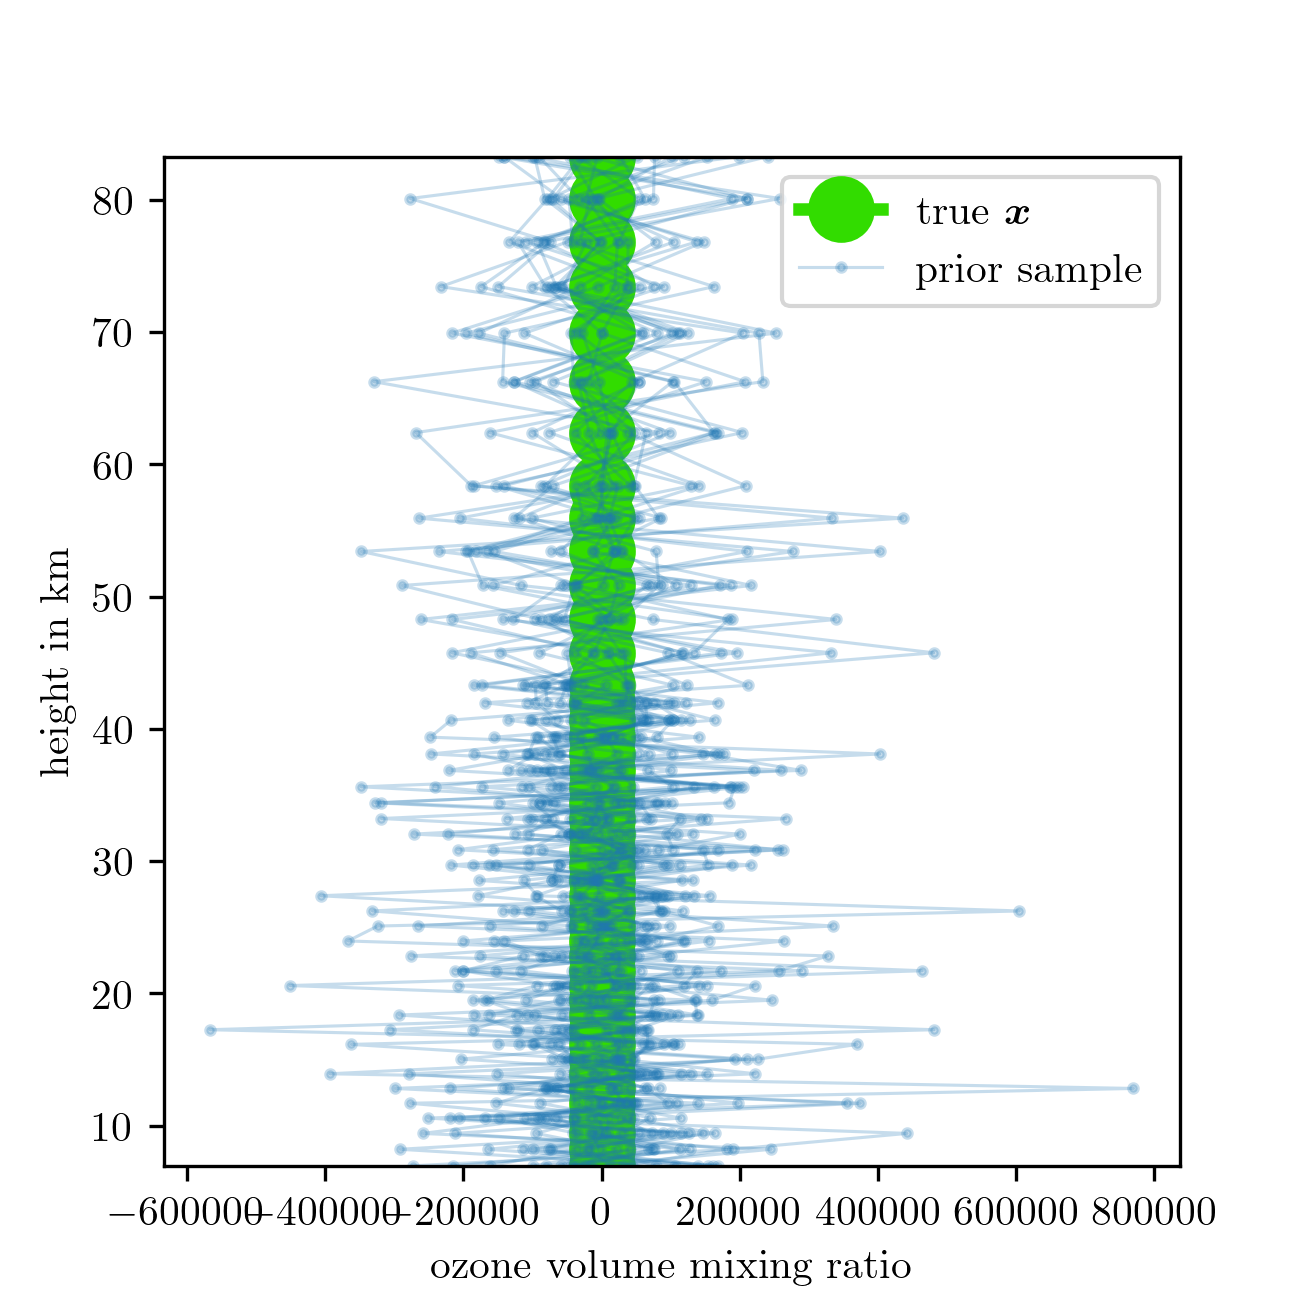
\includegraphics{OzonePrior.png}
	\caption[]{}
	\label{fig:O3Prior}
\end{figure}
\subsubsection{pressure over temperature}


\begin{itemize}
	\item show that pressure is dominant
	\item correlation structure
	\item appendix
\end{itemize}

PriorTempOverPostMeanSigm



\begin{figure}[ht!]
	\centering
	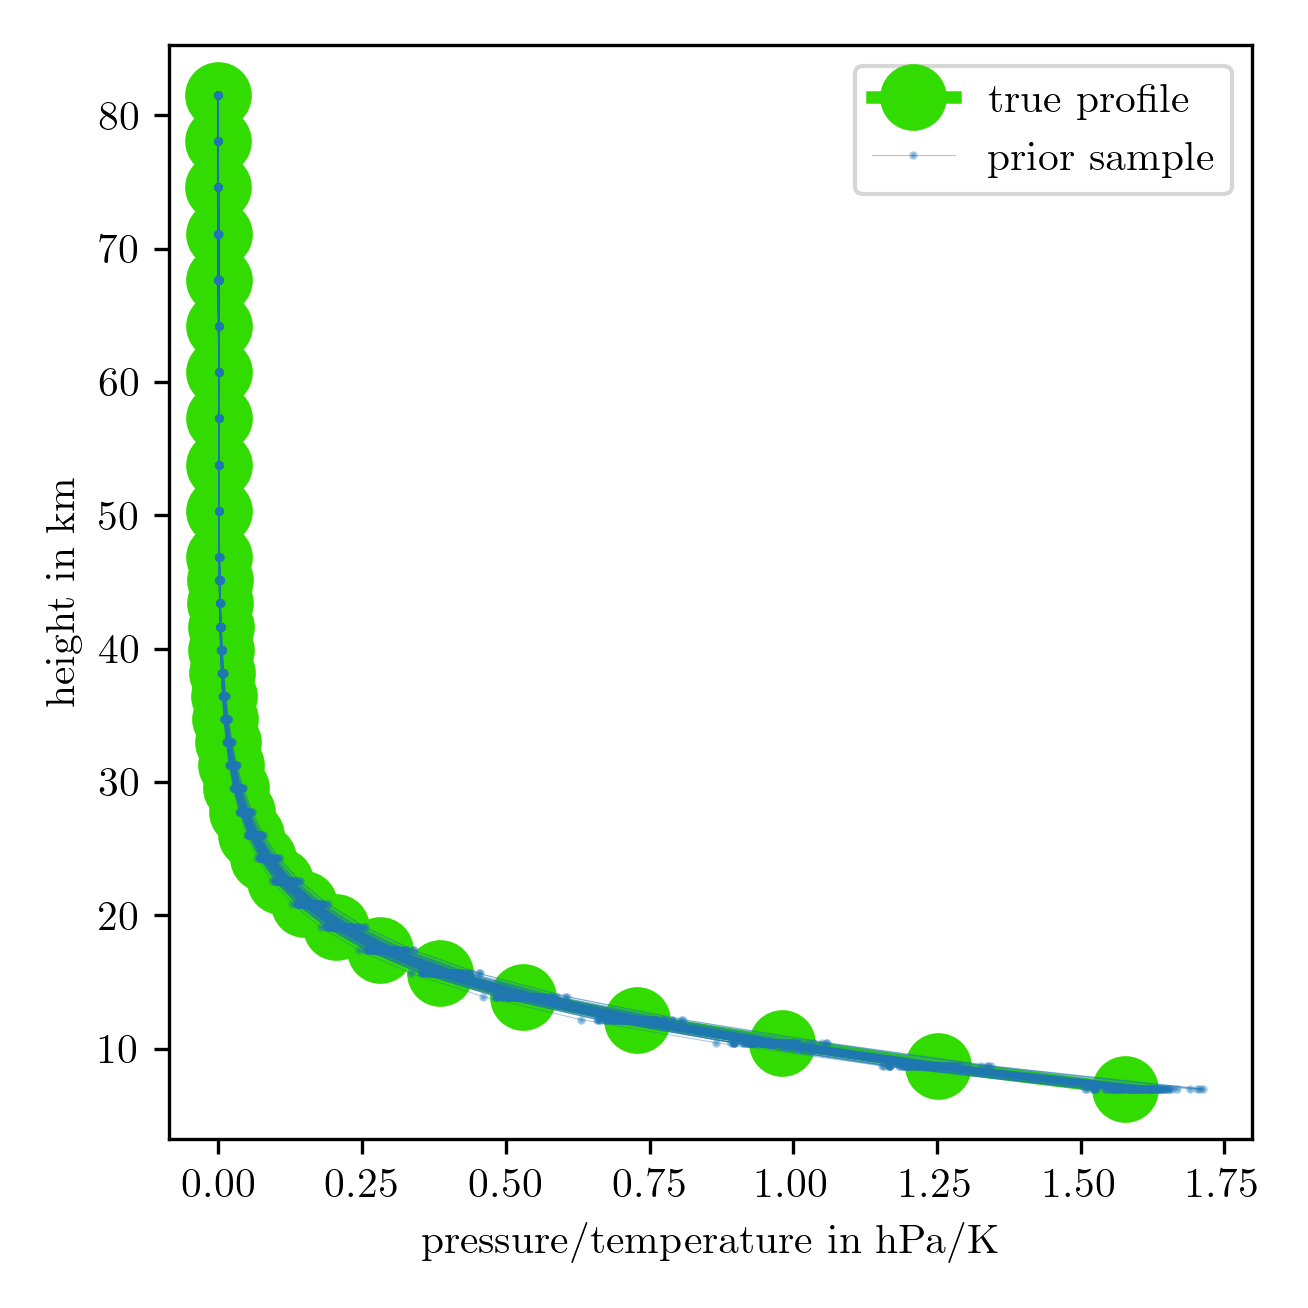
\includegraphics{PriorTempOverPostMeanSigm.png}
	\caption[]{}
	\label{fig:PriorPressOverTemp}
\end{figure}

\begin{figure}[ht!]
	\centering
	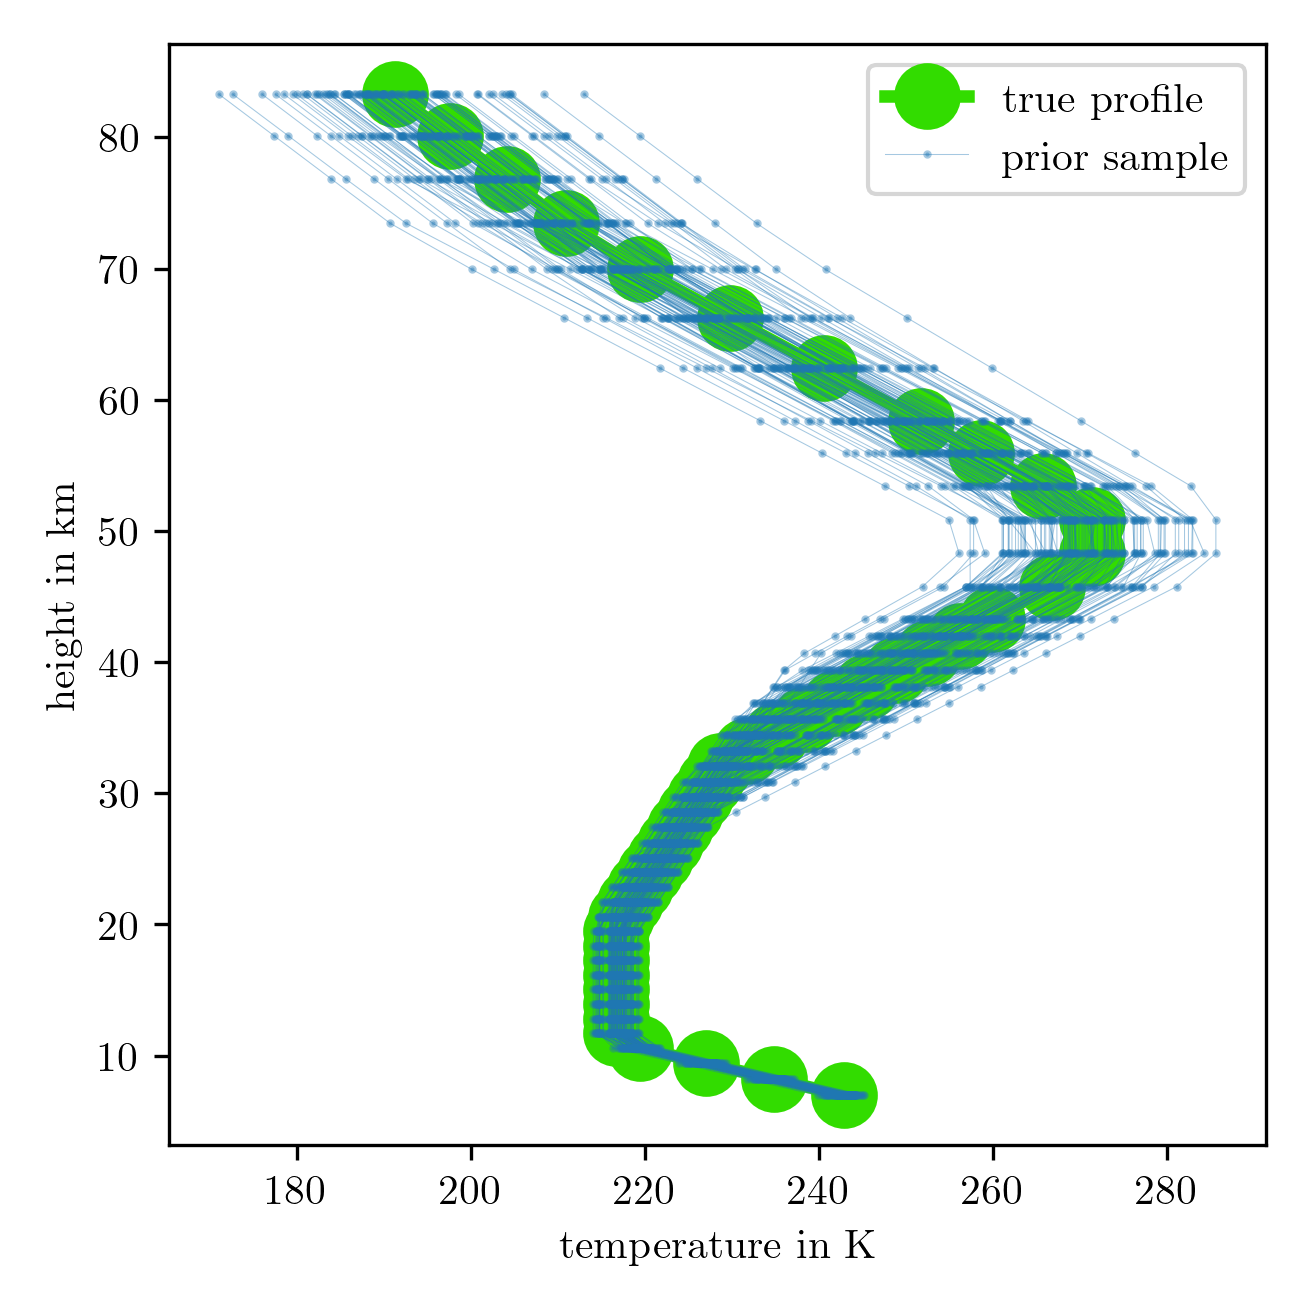
\includegraphics{PriorTempPostMeanSigm.png}
	\caption[]{}
	\label{fig:PriorTemp}
\end{figure}

\begin{figure}[ht!]
	\centering
	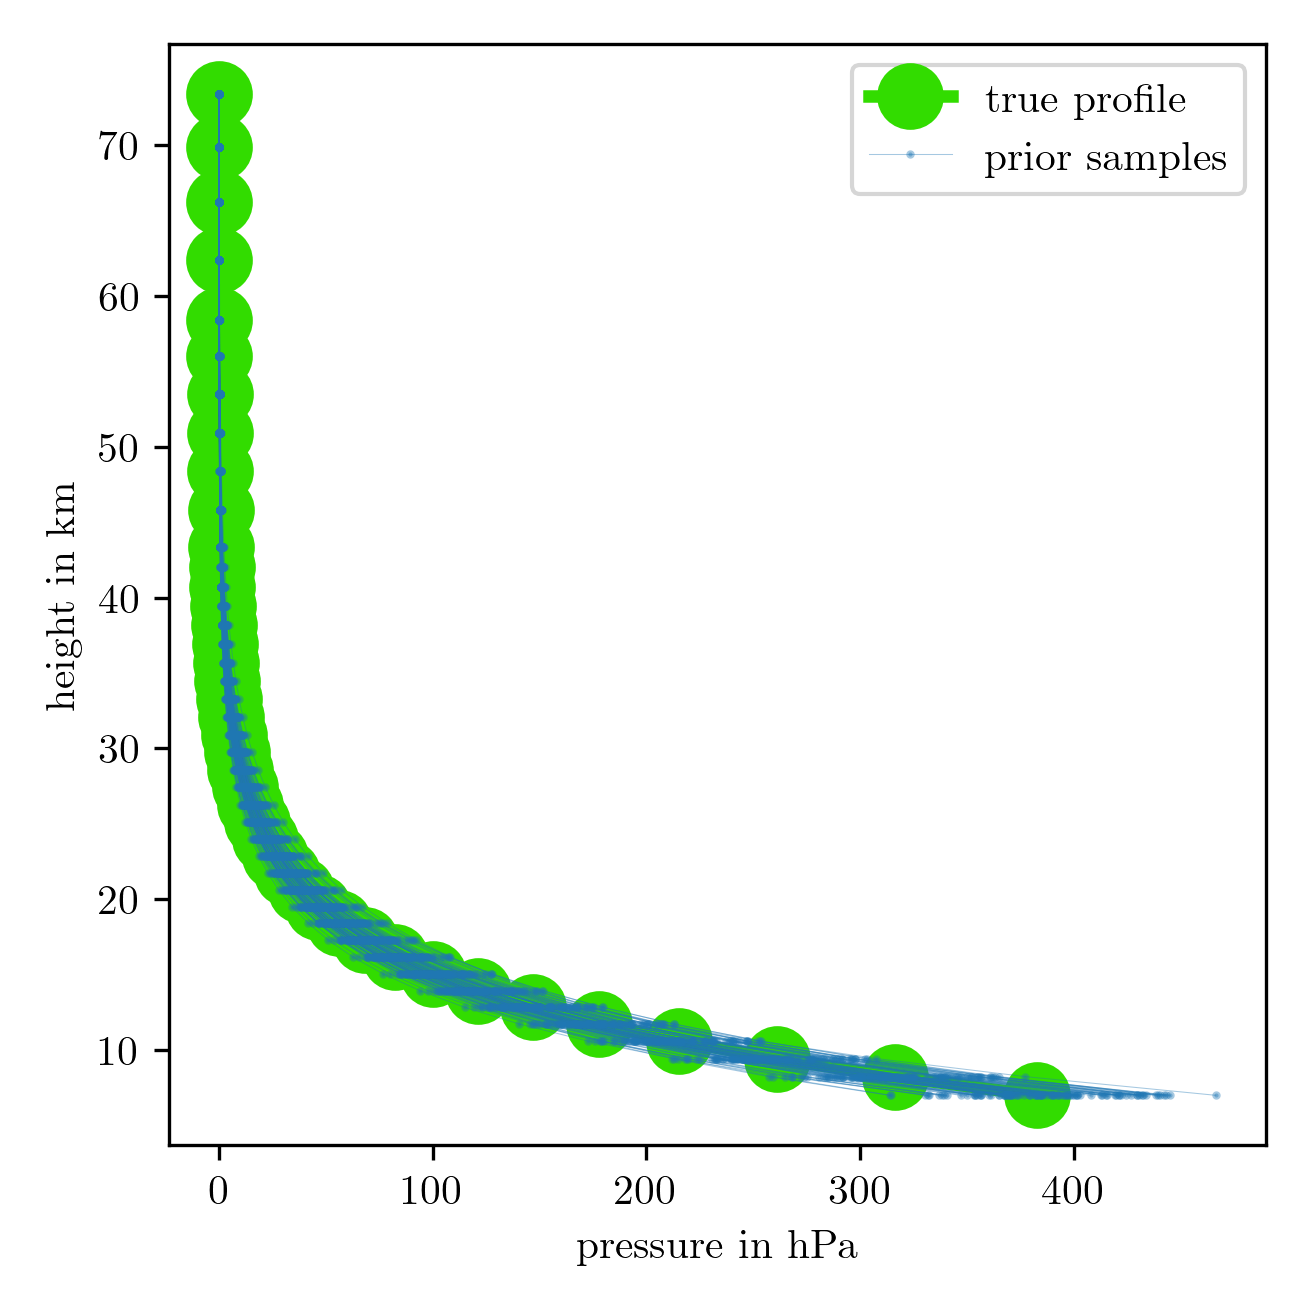
\includegraphics{PriorPressPostMeanSigm.png}
	\caption[]{}
	\label{fig:PriorPress}
\end{figure}


\subsection{Posterior distributions}
\begin{itemize}
	\item explain where we use MTC and that T/p is spereate
	\item marginal posterior, noise and covarince and perciosn matrix
	\item picture of f and g
	\item taylor expansion
	\item maybe make  metroplis explixit
\end{itemize}
conditioned on a ozone profile
\subsubsection{pressure over temperature}

conditioned on a temperauter opver pressure profile
\subsubsection{Ozone -- marginal posterior}
\section{MTC posterior sampling}
\label{sec:postsamp}
In this Section we discuss sampling from the posterior distribution. But you don't need to.
\subsection{Sampling from the marginal posterior distribution over hyper-parameters}
%In this section we present two algorithm to sample from the marginal posterior distribution.
Now, to sample from the marginal posterior of the hyper-parameters
% and the posterior distribution of the parameters condition on the hyper-parameter $\pi(\bm{x}|\bm{y}, \lambda, \gamma )$, with $\lambda = \delta / \gamma$.
\begin{align}
	\pi(\lambda, \gamma | \bm{y})
	\propto  \lambda^{n/2} \gamma^{m/2}   \exp{ \Bigl\{ - \frac{1}{2} g ( \lambda) - \frac{\gamma}{2} f ( \lambda) \Bigr\} } \pi(\lambda, \gamma),
	\label{eq:MargPostAppl}
\end{align}
with $\lambda = \delta / \gamma$,
\begin{subequations}
	\label{eq:fandg}
	\begin{align}
		&f ( \lambda) = \bm{y}^T \bm{y} - (\bm{A}^T \bm{y})^T (\bm{A}^T  \bm{A} + \lambda \bm{L})^{-1} (\bm{A}^T \bm{y})  \, ,  \\
		&\text{and } g(\lambda) = \log \det (\bm{A}^T  \bm{A} + \lambda \bm{L}) \,.
	\end{align}
\end{subequations}
we employ a so-called MWG (Metropolis within Gibbs) algorithm, summarised in the algorithmic Box $1$.
One may implement a Metropolis random walk on the full conditional
\begin{align}
	\label{eq:lamCondPrior}
	\pi(\lambda | \bm{y}, \gamma) &\propto \lambda^{n/2+\alpha_\delta -1} \exp{\Bigl\{ - \frac{1}{2} g ( \lambda) - \frac{\gamma}{2} f ( \lambda) - \beta_\delta \gamma \lambda \Bigr\}} 
\end{align} 
and do a Gibbs steps on
\begin{align}
	\gamma |  \bm{y}, \lambda &\sim \Gamma \bigg( \frac{m}{2} + \alpha_\delta + \alpha_\gamma, \frac{1}{2} f (\lambda ) + \beta_\gamma + \beta_\delta \lambda \bigg)\label{eq:gamCondPrior}
\end{align} 
to generate marginal posterior samples $(\lambda, \gamma)^{(1)}, \dots, (\lambda, \gamma)^{(N)} \sim  \pi(\lambda, \gamma| \bm{y})$.
Note that, when changing variables from $\delta = \lambda \gamma$ to $\lambda$ the hyper-prior distribution changes to $\pi(\lambda) \propto \lambda^{\alpha_\delta-1} \gamma^{\alpha_\delta} \exp{(- \beta_\delta \lambda  \gamma)} $, due to $\text{d}\delta / \text{d} \lambda = \gamma$.
We find the full conditionals by factorisation.



As part of the Metropolis random walk, a new $\lambda^\prime$ given the previous $\lambda^{(k)}$, with $k = 1 , \dots, N$, is proposed according to the distribution $q(\lambda^\prime|\lambda^{(k)}) \sim \mathcal{N}(\lambda^{(k)}, w_\lambda)$.
The proposed sample is rejected or accepted with the acceptance probability $\alpha(\lambda^\prime |\lambda^{(k)})$, see Equation \eqref{eq:alpha}.
Here, calculating the difference $\Delta f = f(\lambda^\prime) - f(\lambda^{(k)})$ and $\Delta g = g(\lambda^\prime) - g(\lambda^{(k)})$ is crucial.
Since the functions $f(\lambda)$ and $g(\lambda)$ are well-behaved over a large range of $\lambda$ and almost linear around the mode of the marginal posterior $\lambda_0$, a Taylor expansion around the mode is sufficient, see Figure \ref{fig:f_and_g}.
Then, computing the acceptance ratio does not involve evaluating $f(\lambda)$ and $g(\lambda)$, but the difference $\Delta f = \sum f^{(r)}(\lambda_0) (\lambda^\prime - \lambda^{(k)})^r$ and $\Delta g = \sum g^{(r)}(\lambda_0) (\lambda^\prime - \lambda^{(k)})^{r}$.
The derivatives are
\begin{align}
	f^{(r)}& (\lambda_0)= (-1)^{r+1} r! (\bm{A}^T \bm{y})^T (\bm{B}_0^{-1} \bm{L})^r \bm{B}_0^{-1} \bm{A}^T \bm{y} \label{eq:ftay}  \\
	\text{and } &g^{(r)} ( \lambda_0) = (-1)^{r+1} \, \text{tr} \big( (\bm{B}_0^{-1}\bm{ L })^r \big)
	\label{eq:gtay}
\end{align} 
with $\bm{B}_0 = \bm{A}^T  \bm{A} + \lambda_0 \bm{L}$.

Finally, a Gibbs step provides a new $\gamma^{(k+1)} \sim \gamma | \bm{y}, \lambda^{(k+1)}$, see Equation \eqref{eq:GibbsStep}.


\subsubsection{Ozone -- conditional posterior}

Conditioned on the hyper-parameters $\bm{\theta} = ( \delta, \gamma)$ we utilise the so-called RTO (randomize then optimize) method \cite{bardsley2012mcmc,bardsley2015randomize, fox2016fast} to draw an independent sample of the conditional posterior distribution.
By perturbation of the exponent of
\begin{align}
	\bm{x}| \bm{y} ,\delta, \gamma \sim \mathcal{N}\big(  (\bm{A}^T \bm{A} + \delta / \gamma \bm{L} )^{-1} \bm{A}^T \bm{y}, (\gamma \bm{A}^T \bm{A} + \delta \bm{L} )^{-1} \big) \, \label{eq:CondPost},
\end{align}
we obtain one independent sample $\bm{x} \sim \pi(\bm{x}|\bm{y}, \bm{\theta})$ for each solve of Equation \eqref{eq:RTO}, see algorithmic Box $2$.


We use the same discretization of the atmosphere as given by the ozone profile taken from \url{https://disc.gsfc.nasa.gov/datasets/ML2O3_005/summary?keywords=mls%20o3}.
We use ozone values between a height of $10$km up to $38$km, which results in $n=37$ layers.
We set the number of measurements to $m= 105 $.
(I can't think of any good reason why I chose that, it is a good number not too big not too small and gives consistent results for various datasets)\\

When finding the mode we use the scipy.optimize.fmin function and limit the number of function evaluations to 25.
We use Cholesky factorisation to evaluate $g(\lambda)$ and $f(\lambda)$ and to construct the coefficients of the Taylor series, where we have to calculate  $\bm{B}^{-1} \bm{L} $ and  $\bm{B}^{-1}  \bm{A}^T \bm{y}$ once at $\lambda_0$.\\


We bin the samples into a normalised histogram and use the height of the bars as quadrature weights $\pi(\lambda_i| \bm{y})$, where the quadrature point $\lambda_i$ denotes the centre of each bin.
To calculate the conditional posterior mean we use approximate quadrature
\begin{align}
	\mu_{\bm{x}|\bm{y}} = \int x_{\lambda} \pi(\lambda| \bm{y}) \text{d}\lambda \approx \sum x_{\lambda_i} \pi(\lambda_i| \bm{y}) \, ,
\end{align}
with $\sum \pi(\lambda_i| \bm{y}) = 1$, so that the integral can be interpreted as the weighted average.
See Sec. 2 \url{https://www.cambridge.org/core/journals/acta-numerica/article/highdimensional-integration-the-quasimonte-carlo-way/03F126DDF465F915B22D5D709CD28946}.\\

We bin the samples into $3$ bins and stop increasing the number of bins by one if the relative error between the previous and the current conditional posterior mean is less than $0.1\%$.
This gives a total number of $3+4+5 = 12$ solves for $x_{\lambda}$.
In addition, we calculate the covariance matrix $(\gamma \bm{B}_{\lambda})^{-1} $, where we use Cholesky factorisation to invert $\bm{B}$, solving the integral
\begin{align}
	\Sigma_{\bm{x}|\bm{y}} = \int \gamma^{-1}  \pi(\gamma | \bm{y} ) \, \text{d} \gamma \, \int  \bm{B}_{\lambda}^{-1} \, \pi(\lambda | \bm{y} )  \, \text{d} \lambda  \approx \sum {\gamma_i}^{-1}\pi(\gamma_i| \bm{y}) \sum \bm{B}_{\lambda_i}^{-1}\pi(\lambda_i| \bm{y})\, .
\end{align}\\

It takes us less than 0.1s to draw 10000 samples from the marginal posterior and to calculate the conditional posterior mean or to solve for 200 different $x_{\lambda}$ and to find the regularised solution at the point of maximum curvature using the kneedle algorithm.\\


\section{Affine Map}
\begin{itemize}
	\item introduce affine sapce and how we get affine map, to motivate samples from posterir space
	\item explicit, why we need ozone profiles, because it is faster and temperature and pressure are more well defined within the atmosphere
	\item generate affine space every samples is a feasable sample
	\item generate data without noise to find affine map
\end{itemize}
We do MTC with linear forward map no updadeted
In this specific case we find the affine map
\begin{align}
	\bm{M} = \begin{bmatrix}
		\text{---} & \bm{M}_0 &   \text{---}  \\
		&  \vdots  & \\
		\text{---}& \bm{M}_j &  \text{---} \\
		&  \vdots  & \\
		\text{---} & \bm{M}_m &   \text{---}
	\end{bmatrix} \, \in \mathbb{R}^{m \times m} ,
\end{align}
with rows $\bm{M}_j$ using a linear solver for
\begin{align}
	W \bm{M}_j^\top \, = V_{j} \, .
\end{align}
Here $V_j$ denotes the $j$th row of  
\begin{align}
	V = \begin{bmatrix}
		\vert&   &  \vert & & \vert \\
		\bm{A}_{NL} (\bm{x}^{(1)} ) &  \cdots& \bm{A}_{NL} (\bm{x}^{(j)} )&  \cdots & \bm{A}_{NL} (\bm{x}^{(m)})  \\
		\vert&   &  \vert & & \vert 
	\end{bmatrix}
\end{align}
and
\begin{align}
	W = \begin{bmatrix}
		\vert&   &  \vert & & \vert \\
		\bm{A}_{L} \bm{x}^{(1)} &  \cdots& \bm{A}_{L} \bm{x}^{(j)} &  \cdots & \bm{A}_{L} \bm{x}^{(m)} \\
		\vert&   &  \vert & & \vert 
	\end{bmatrix}
\end{align}
is a $\mathbb{R}^{m \times m} $ matrix as well as $\bm{A}_{NL}$.
Then the non-linear forward model can be approximated so that
\begin{align}
	\bm{A}_{NL}(\bm{x}) \approx \bm{M A}_L \bm{x}\, .
\end{align}

\subsection{First MTC}
\begin{itemize}
	\item make table with set up for TT and sampling , number of samples
	\item normalize in evrey step
	\item we use RTO to generate samples
\end{itemize}
\begin{figure}[thb!]
	\centering
	\begin{tikzpicture}
	\node[roundnode2] at (-4.5,6.5) (Q)     {$\bm{Q}$};
	\node[roundnode2] at (-3,5) (x)     {$\bm{x}$};
	\node[align=center] at (-1.55,4) (A)    {$\bm{A}_L$};
	\node[roundnode2] at (-1.55,2.5) (u)    {$\bm{u}$};
	\node[rectnode] at (-1.55,1) (y)    {$\bm{y}$};
	\node[roundnode2] at (-5.25,4.5) (S)    {$\bm{\Sigma}$};
	\node[roundnode2] at (-6.5,6.25) (s)    {$\gamma$};
	\node[roundnode2] at (-5.5,8) (d)    {$\delta$};
		
	%Lines
	\draw[->, mydotted, very thick] (S.south east) -- (y.west);
	\draw[->, very thick] (s.south) -- (S.north west);
	\draw[->, very thick] (u.south) -- (y.north);
	\draw[->, mydotted, very thick] (A.south) -- (u.north);
	\draw[->, mydotted,  very thick] (x.south east) -- (A.west);
	
	\draw[->, very thick] (d.south) -- (Q.north west); 
	
	\draw[->, very thick] (Q.south east) -- (x.north west); 
	%\node[align=center] at (0,4) (f3) {$= \bm{A}$};
	%\node[align=center] at (0.25,3.95) (f3) {$\approx \bm{M A}_L$};
	\node[align =center] at (-1.75,7) (T1) {marginal posterior \\ over hyper-parameters \\ $\pi(\gamma, \delta | \bm{y})$};
	\node[align =center] at (-0.75,5) (T1) {conditional posterior \\ $\pi( \bm{x} |\gamma, \delta, \bm{y})$ };

	
	\node[fit=(S)(s)(Q)(d),draw,dotted,black, rounded corners] {};
	\end{tikzpicture} 
\caption[]{}
\end{figure}

\subsubsection{Marginal Posterior}
\begin{itemize}
	\item samples vs calc values
	\item taylor expansion
\end{itemize}

\begin{figure}[ht!]
	\centering
	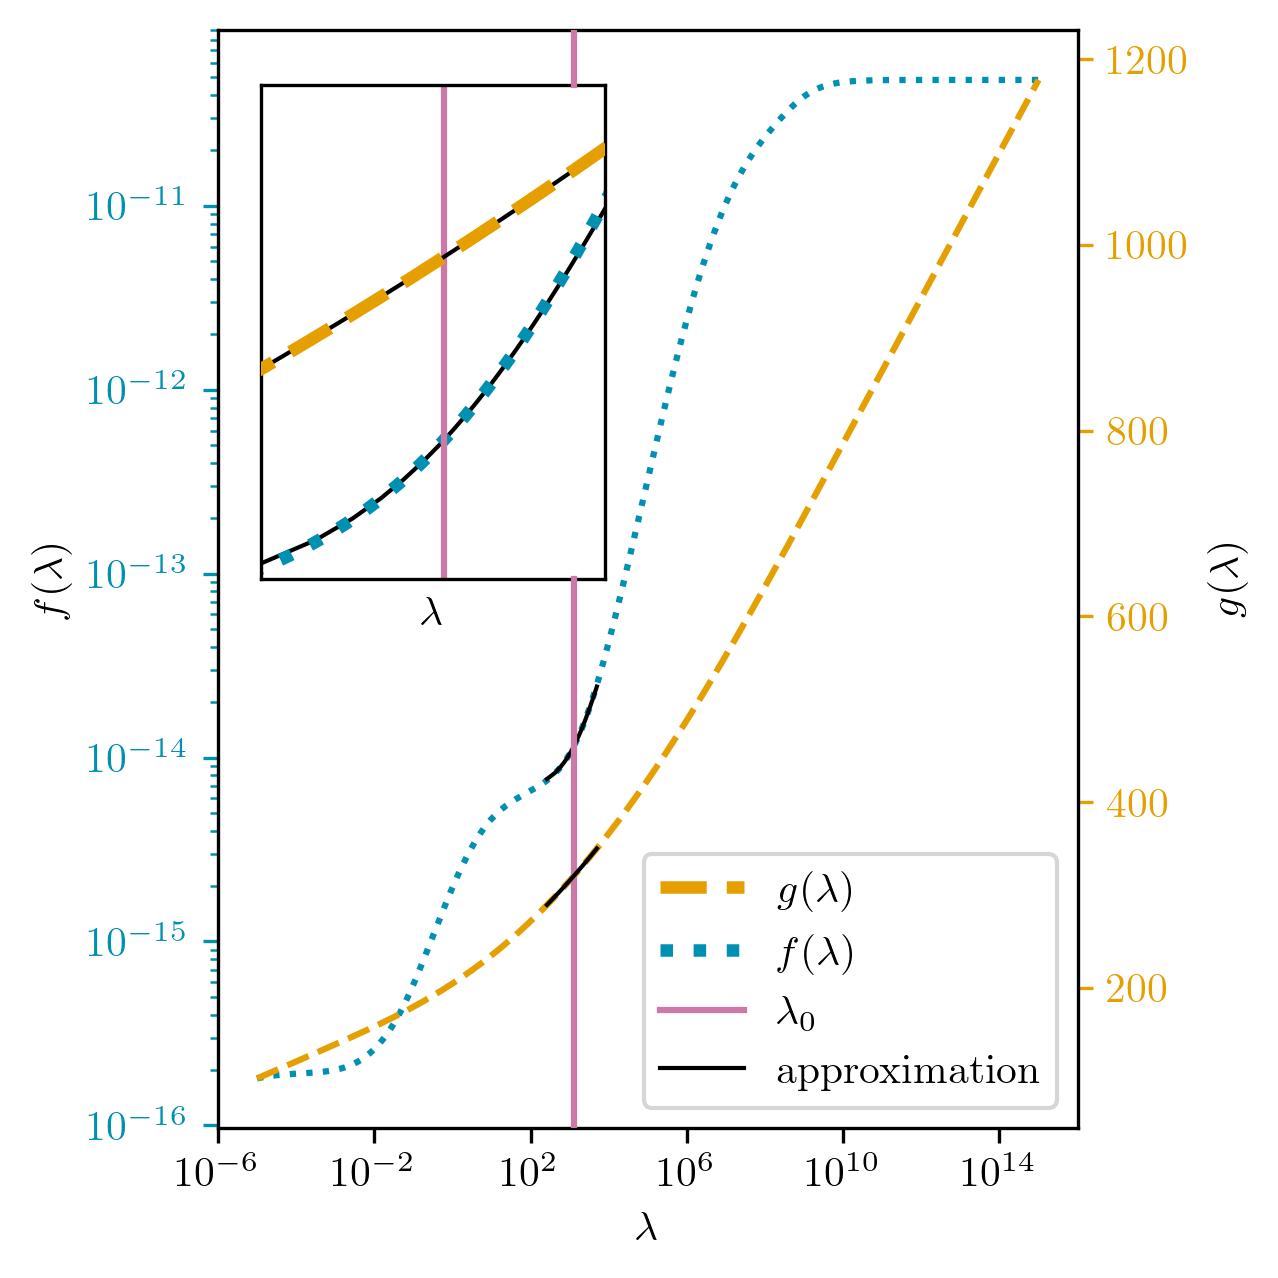
\includegraphics{f_and_g_phd.png}
	\caption[]{}
	\label{fig:fandg}
\end{figure}

%\begin{figure}[ht!]
%	\centering
%	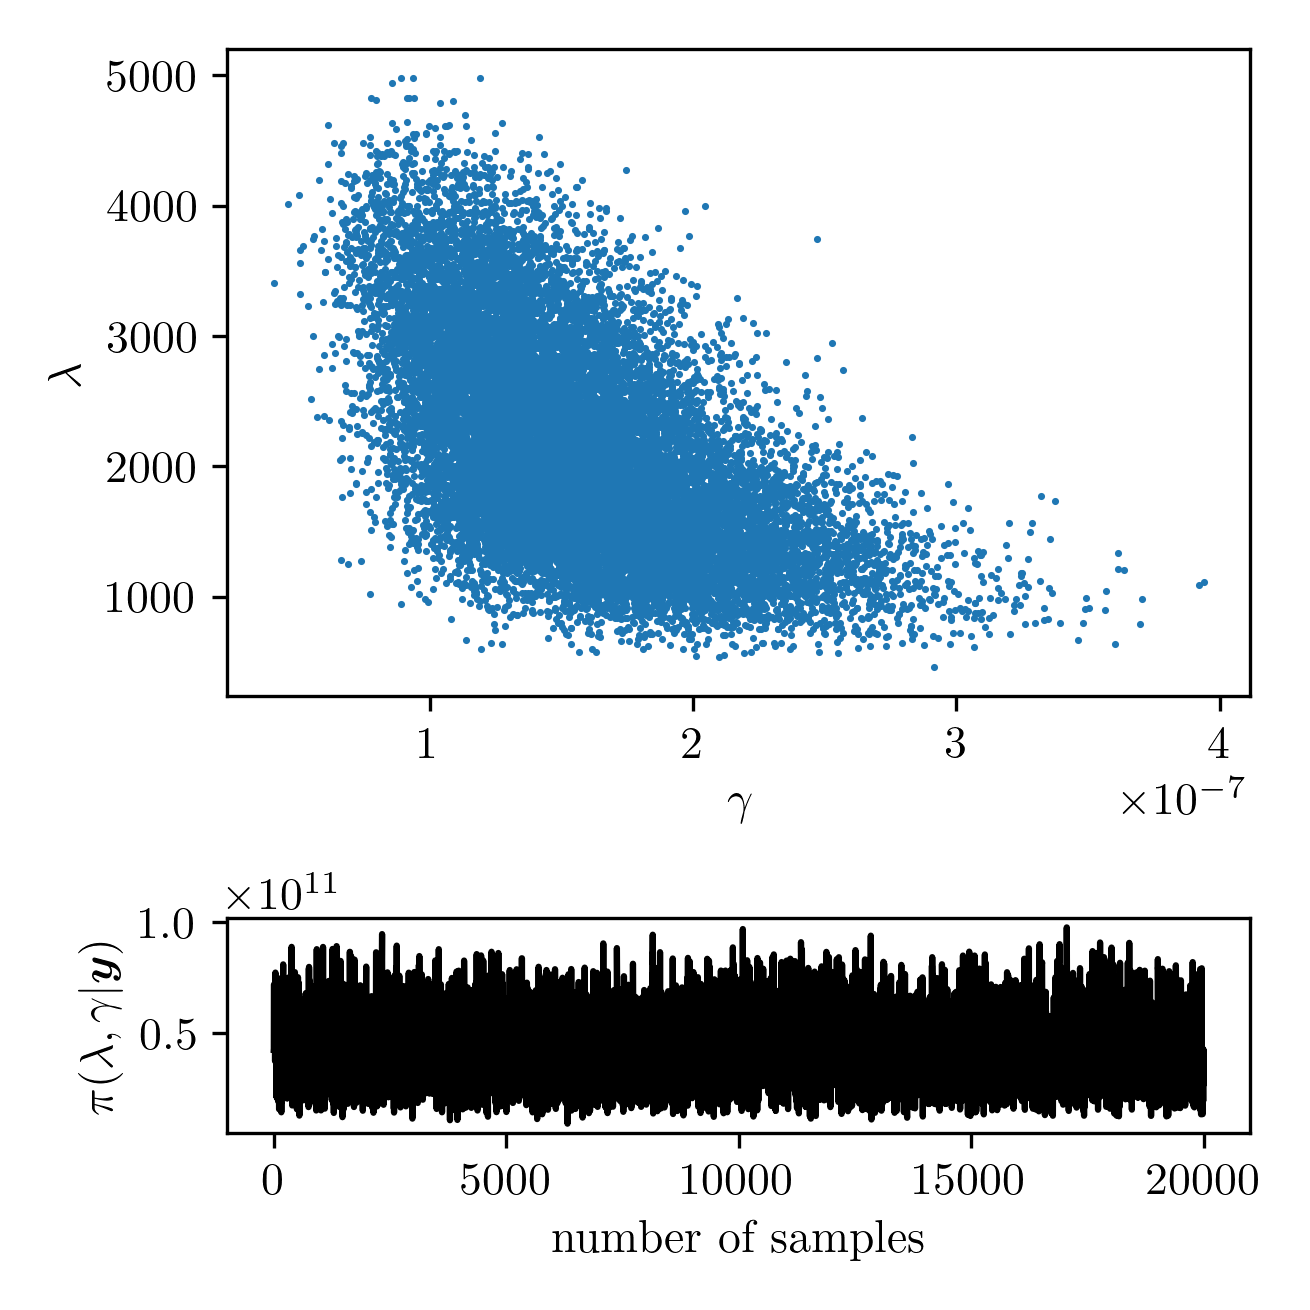
\includegraphics{ScatterplusHisto.png}
%	\caption[]{}
%	\label{fig:}
%\end{figure}

\begin{figure}[ht!]
	\centering
	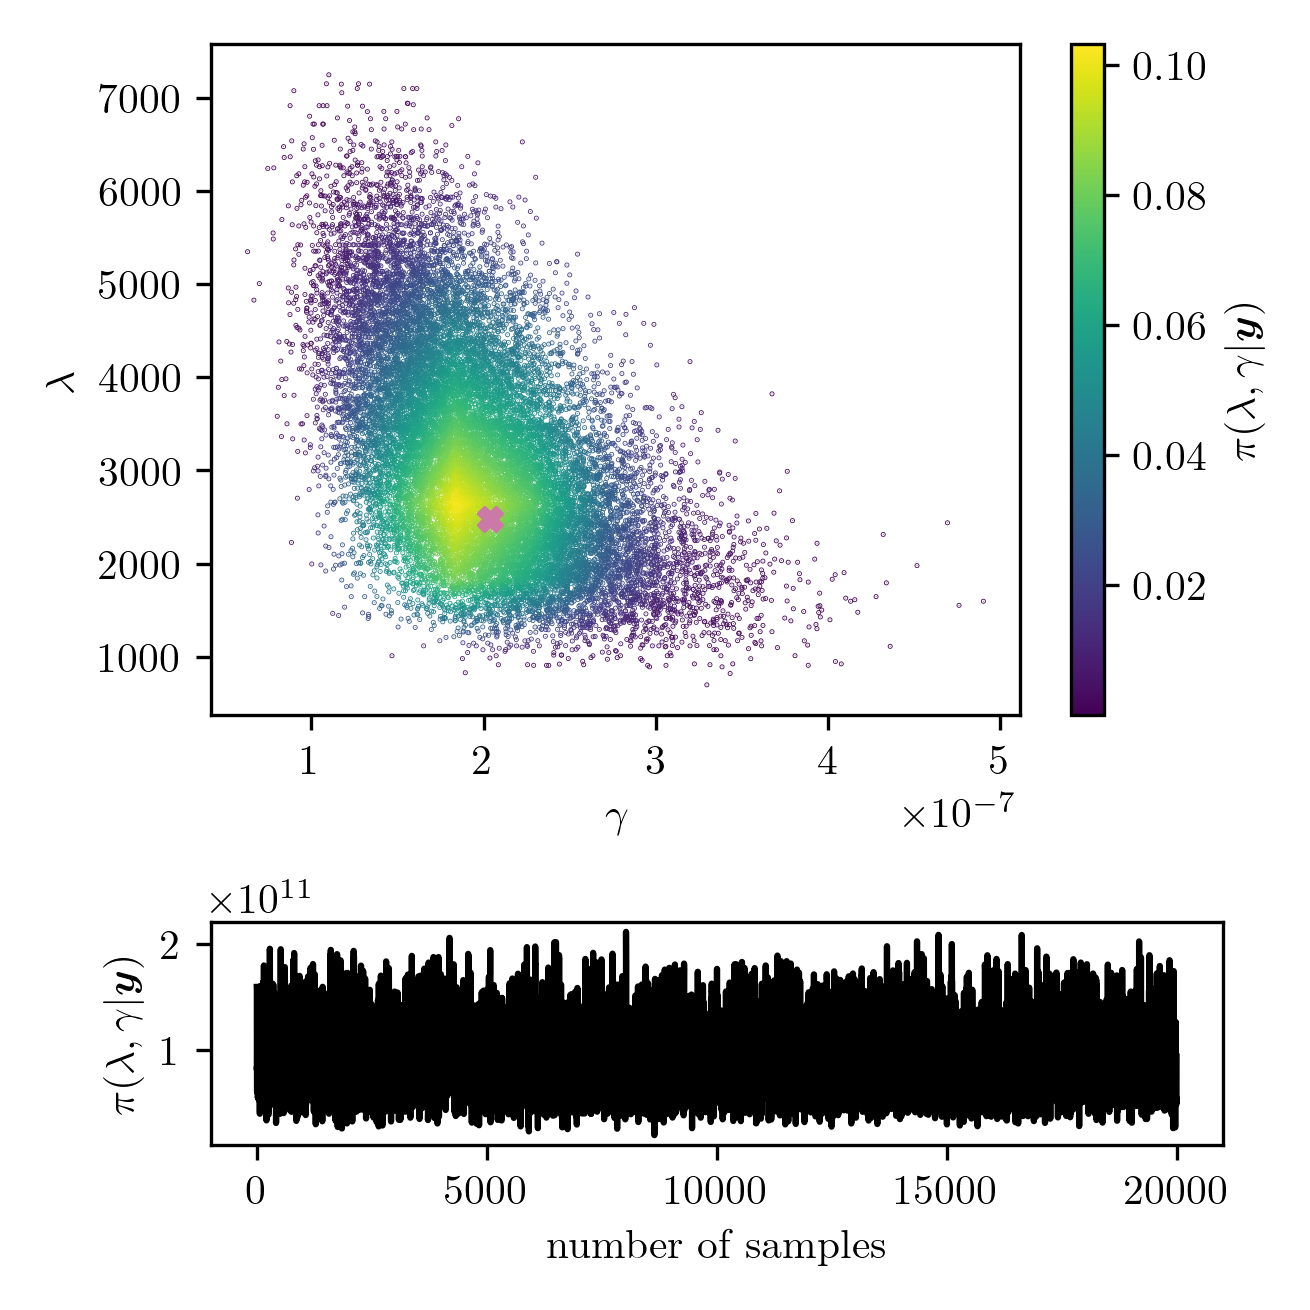
\includegraphics{ScatterplusHistoPlusTT.png}
	\caption[]{}
	\label{fig:ScatterPlotTT}
\end{figure}


\subsubsection{sampling from conditional posterior Posterior}
\begin{itemize}
	\item draw samples using RTO no need to calc variance yet, when variance is hard to calculate, we use cholesky defactorization (maybe put in appendix)
	\item or calc mean and variance using see other section
\end{itemize}
\begin{figure}[ht!]
	\centering
	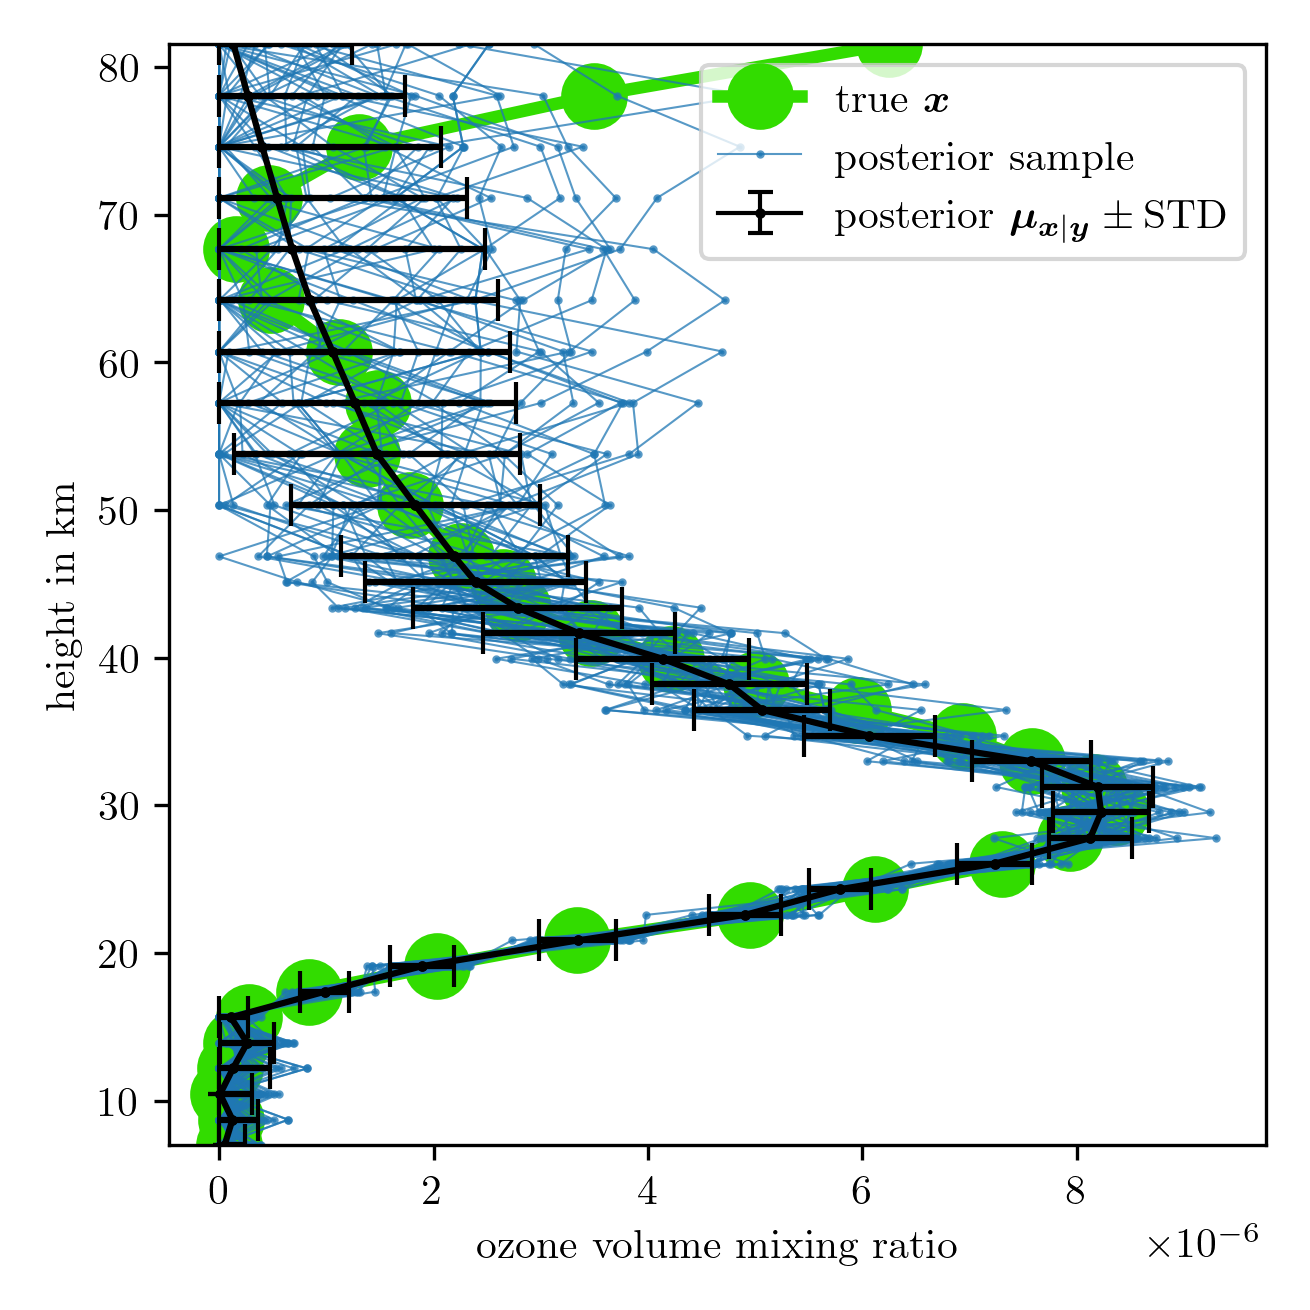
\includegraphics{FirstTestRes.png}
	\caption[]{}
	\label{fig:O3Samp}
\end{figure}


\subsection{Generate and Asses Affine Map}
\begin{figure}[ht!]
	\centering
	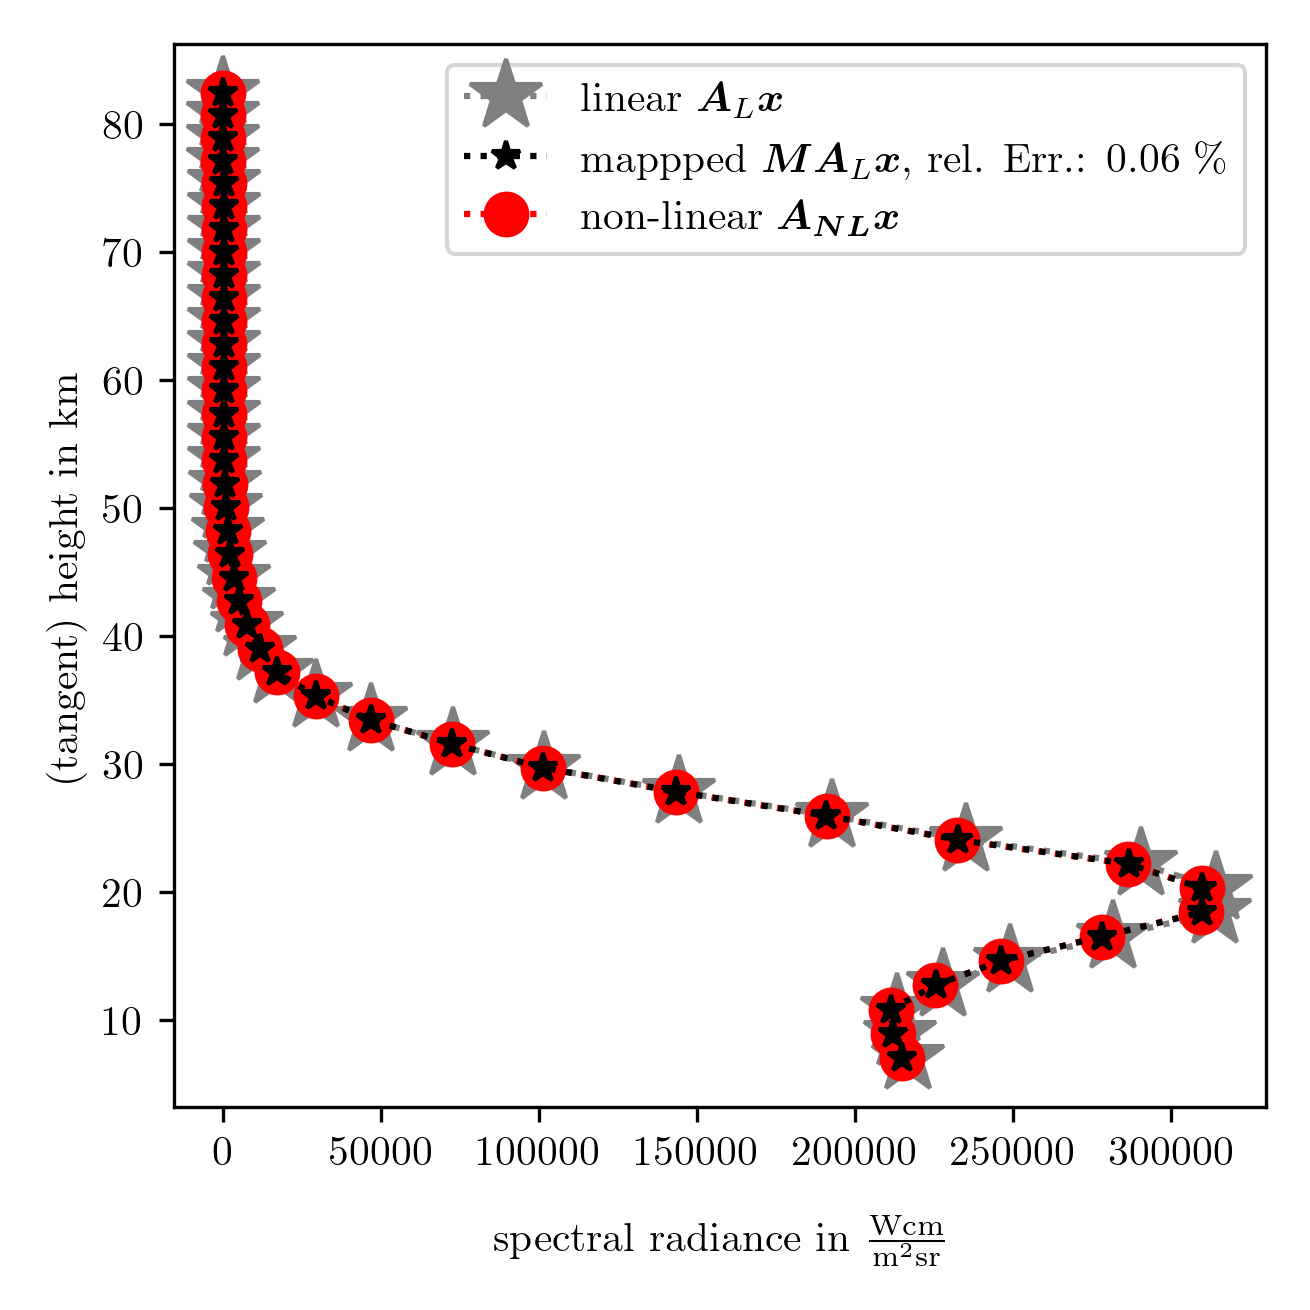
\includegraphics{SampMapAssesment.png}
	\caption[]{}
	\label{fig:MapAsses}
\end{figure}


\section{Updated Forward map}

\begin{itemize}
	\item updated forward map
	\item do mtc again but this time with weighted integration and then condition on pressure and temperature, samples
	\item for sake of completeness regularised solution and say disadvantage, maybe include in table
\end{itemize}


\subsection{Ozone Retrieval}
%\begin{figure}[ht!]
%	\centering
%	\includegraphics{secRecRes.png}
%	\caption[]{}
%	\label{fig:}
%\end{figure}

\subsubsection{MTC --  sampling vs TT}
\begin{figure}[ht!]
	\centering
	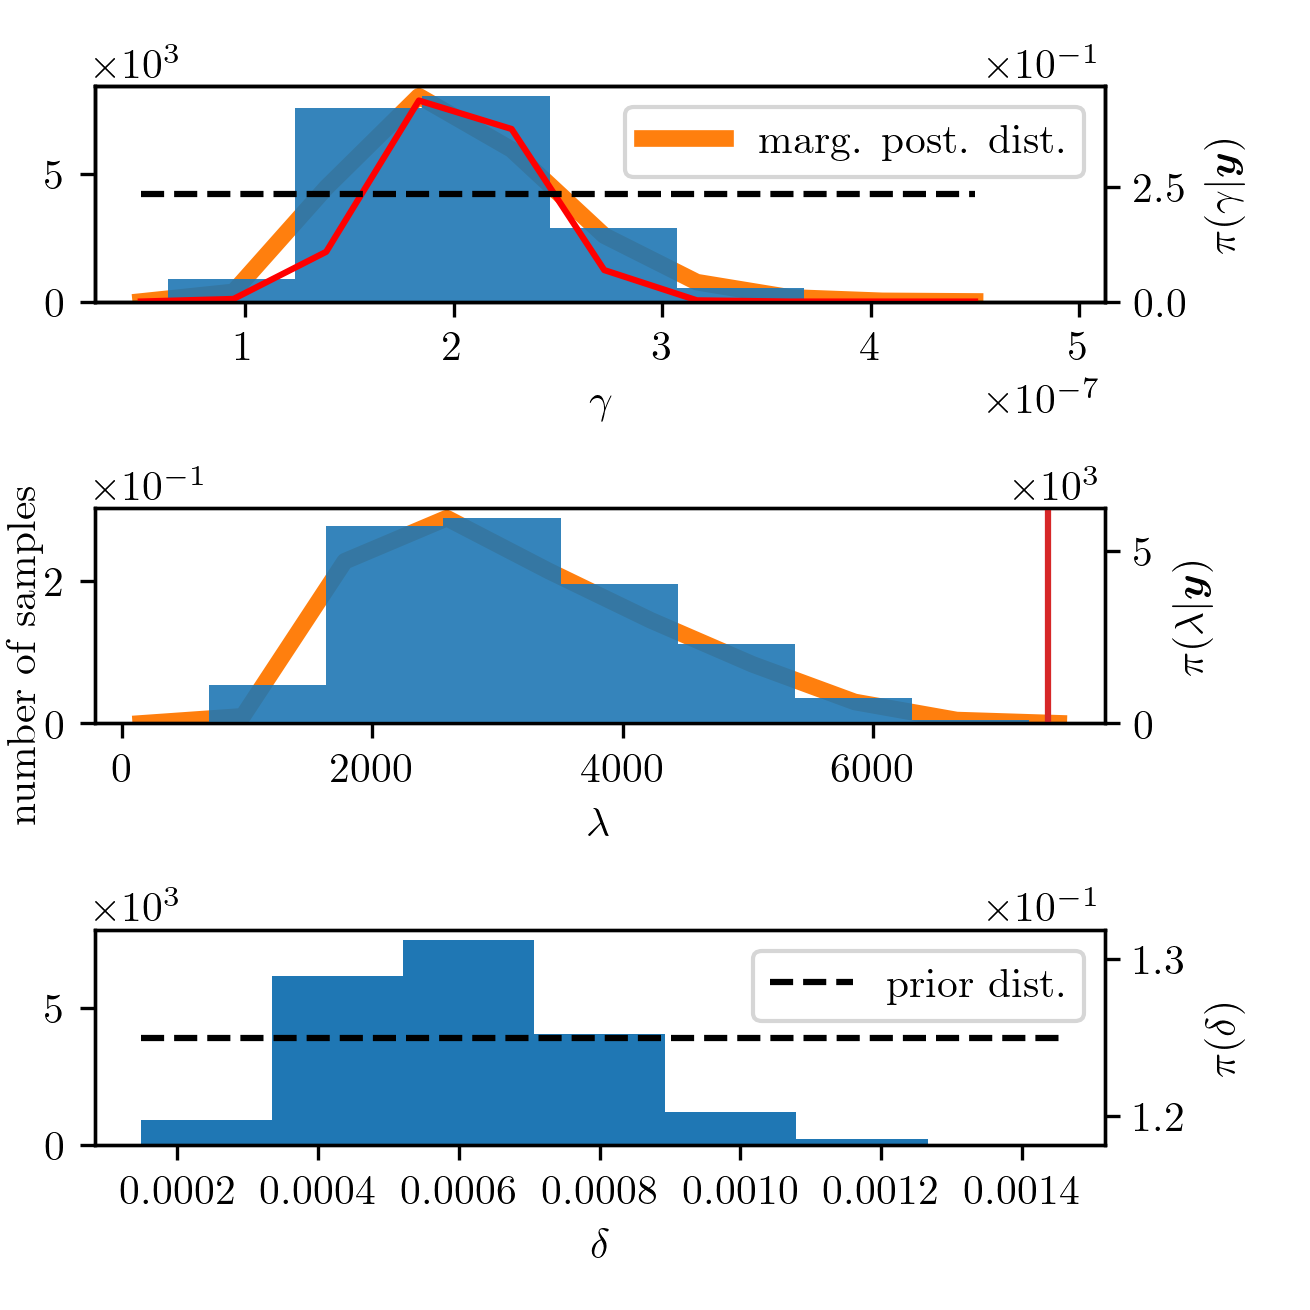
\includegraphics{secSIRTMargMargO3Res.png}
	\caption[]{}
	\label{fig:MargPostHistTT}
\end{figure}
\subsubsection{Regularized Solution}
\begin{itemize}
	\item similar to MTC model
	\item picture of L-Curve and samples 
	\item include in reg paraemter in histograms
\end{itemize}
\begin{figure}[ht!]
	\centering
	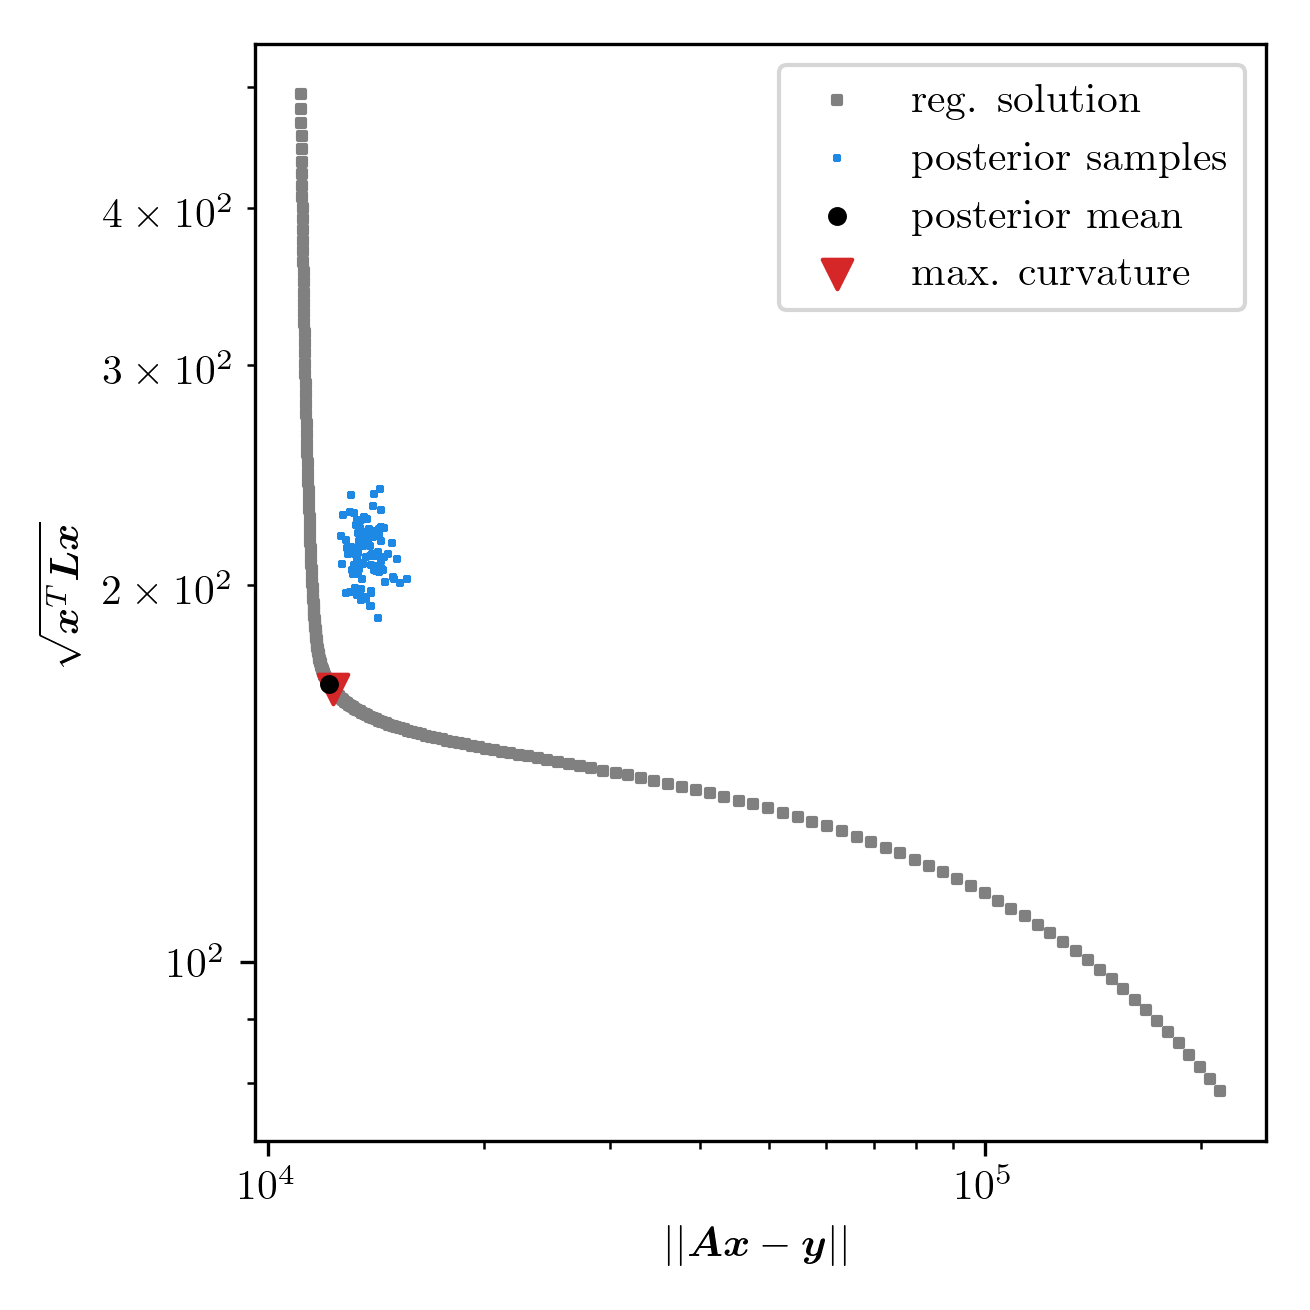
\includegraphics{LCurvePhD.png}
	\caption{We take the ozone profile from \cite{}, relate pressure and height and discretise according to the source.
		This will serve as our true Ozone profile.}
	\label{fig:LCurve}
\end{figure}

\begin{figure}[ht!]
	\centering
	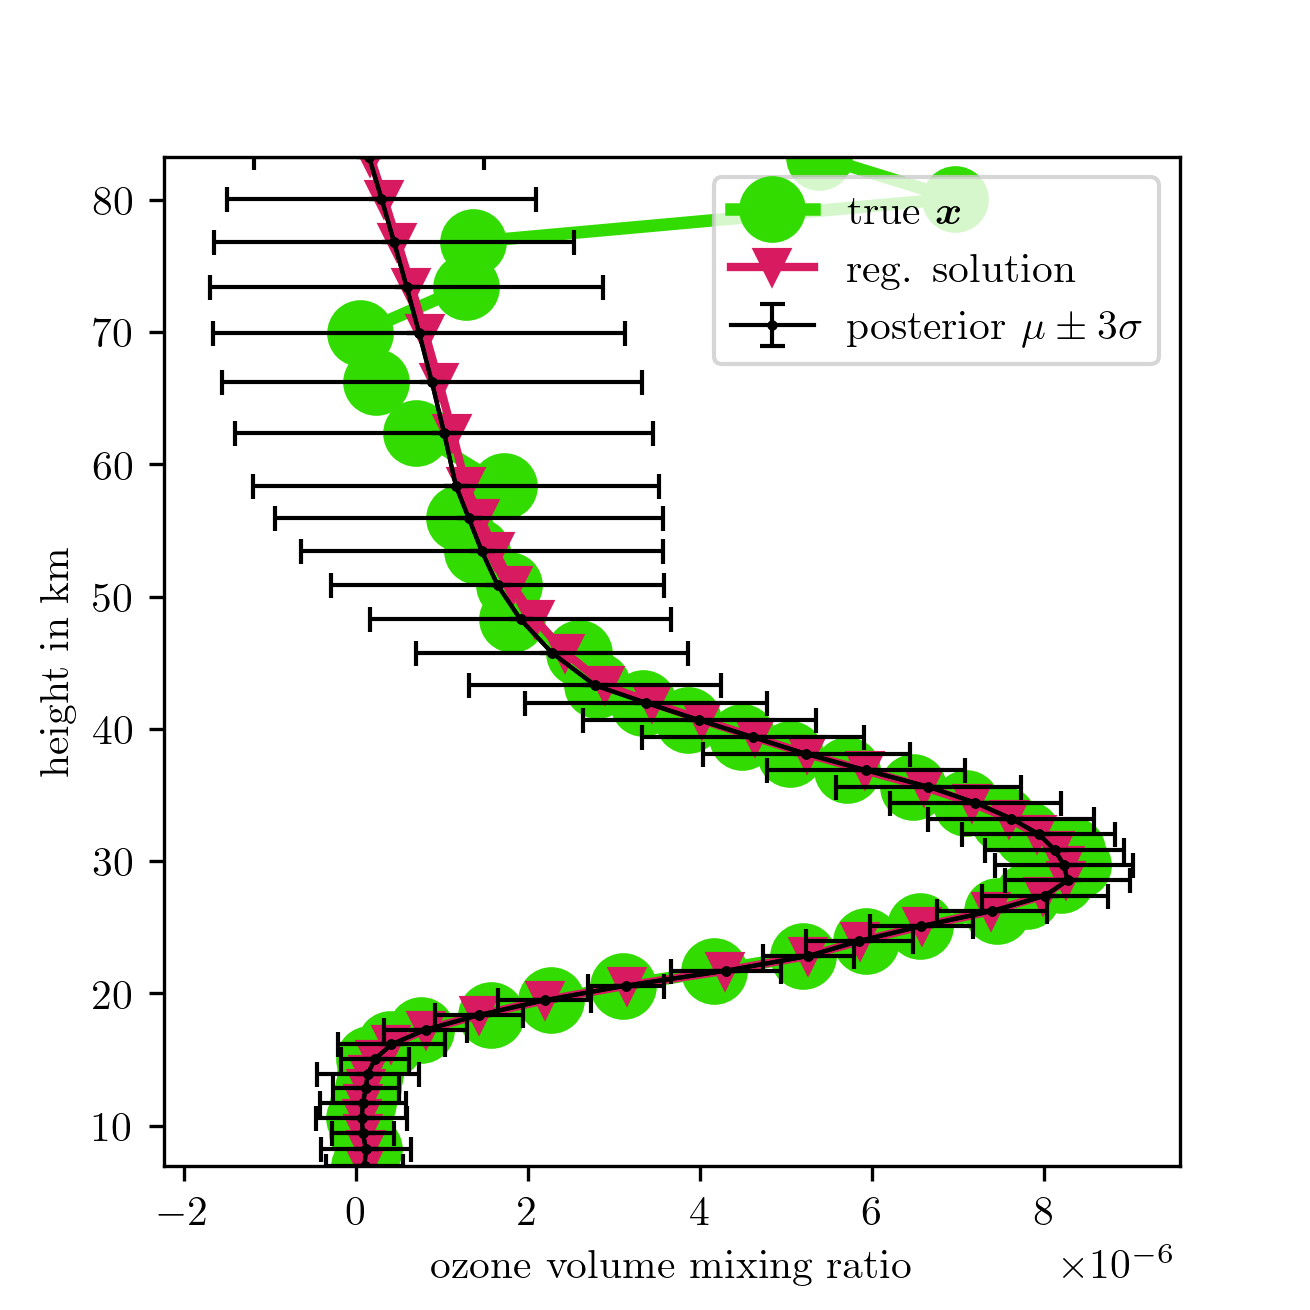
\includegraphics{SecRecResinclReg.png}
	\caption[]{}
	\label{fig:O3SolplsReg}
\end{figure}




\subsection{Posterior Pressure and Temperature}
\begin{itemize}
	\item make table with set up for TT and sampling t-walk
\end{itemize}
\begin{figure}[thb!]
	\centering
	\begin{tikzpicture}
		
		\node[align=center] at (-1,4) (A)    {$\bm{M A}_L$};
		\node[roundnode2] at (-1,2.5) (u)    {$\bm{u}$};
		\node[rectnode] at (-1,1) (y)    {$\bm{y}$};
		
		\node[roundnode2] at (3,6.5) (t)     {$\bm{T}$};
		\node[roundnode2] at (-1,6.5) (p)     {$\bm{p}$};
		\node[roundnode2] at (1,5) (pt)     {$\bm{p}/\bm{T}$};
		\node[roundnode2] at (0,8) (b1)    {$b$};
		%\node[roundnode2] at (1,8) (b2)    {$b_2$};
		\node[roundnode2] at (-2,8) (h1)    {$h_0$};
		\node[roundnode2] at (-1,8) (p0)    {$p_0$};
		\node[roundnode2] at (2.25,8) (ht)    {$\bm{h}$};
		\node[roundnode2] at (3.25,8) (ct)    {$T_0$};
		\node[roundnode2] at (4.25,8) (at)    {$\bm{a}$};
		
		%Lines
		\draw[->, very thick] (u.south) -- (y.north);
		\draw[->, mydotted, very thick] (A.south) -- (u.north);
		
		\draw[->, mydotted, very thick] (p.south east) -- (pt.north west);
		\draw[->, mydotted, very thick] (t.south west) -- (pt.north east);
		\draw[->, mydotted, very thick] (pt.south west) -- (A.east);
		\draw[->, mydotted, very thick] (h1.south) -- (p.north west);
		\draw[->, mydotted, very thick] (p0.south) -- (p.north);
		\draw[->, mydotted, very thick] (b1.south) -- (p.north east); 
		%\draw[->, very thick] (b2.south) -- (p.east); 
		
		\draw[->, mydotted, very thick] (ht.south) -- (t.north west);
		\draw[->, mydotted, very thick] (ct.south) -- (t.north);
		\draw[->, mydotted, very thick] (at.south) -- (t.north east);
		
		\node[align =center] at (-5,8) (T1) {posterior \\ over hyper-parameters \\ $\pi(h_0, p_0, b, \bm{h}, T_0, \bm{a}| \bm{y})$};
		
		\node[fit=(h1)(at),draw,dotted,black, rounded corners] {};
	\end{tikzpicture} 
\caption[]{}
\end{figure}

\begin{figure}[ht!]
	\centering
	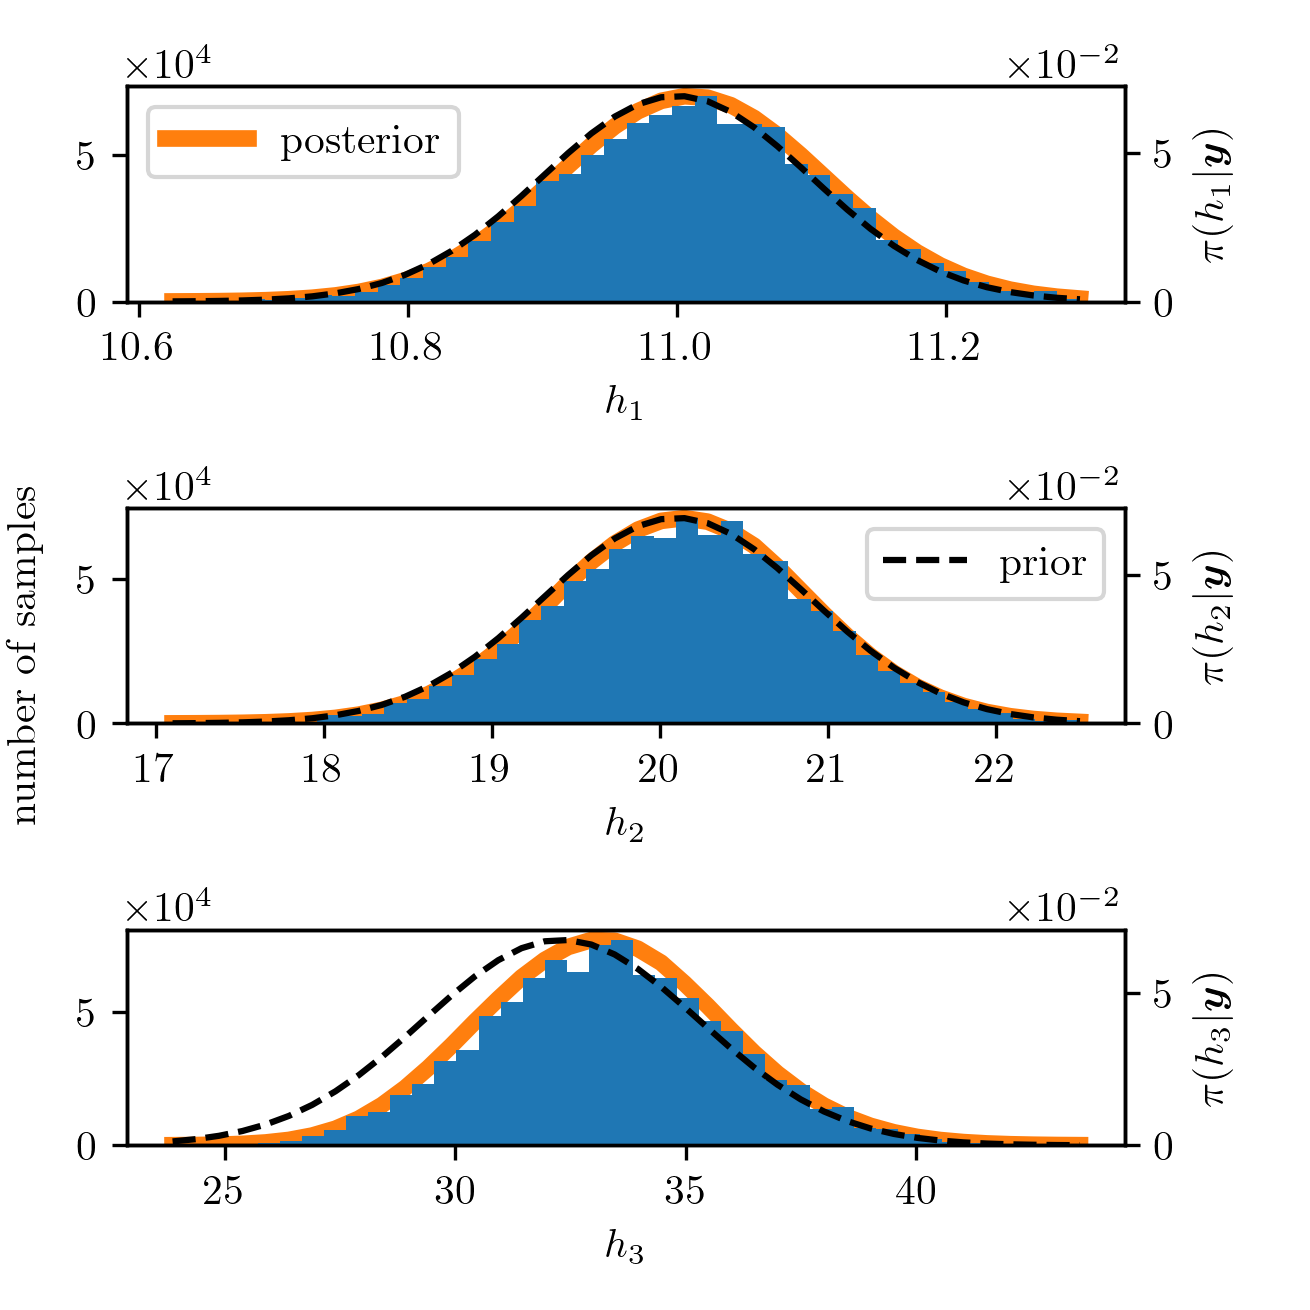
\includegraphics{PHdPTPost0.png}
	\caption[]{}
	\label{fig:PostHistTT0}
\end{figure}
\begin{figure}[ht!]
	\centering
	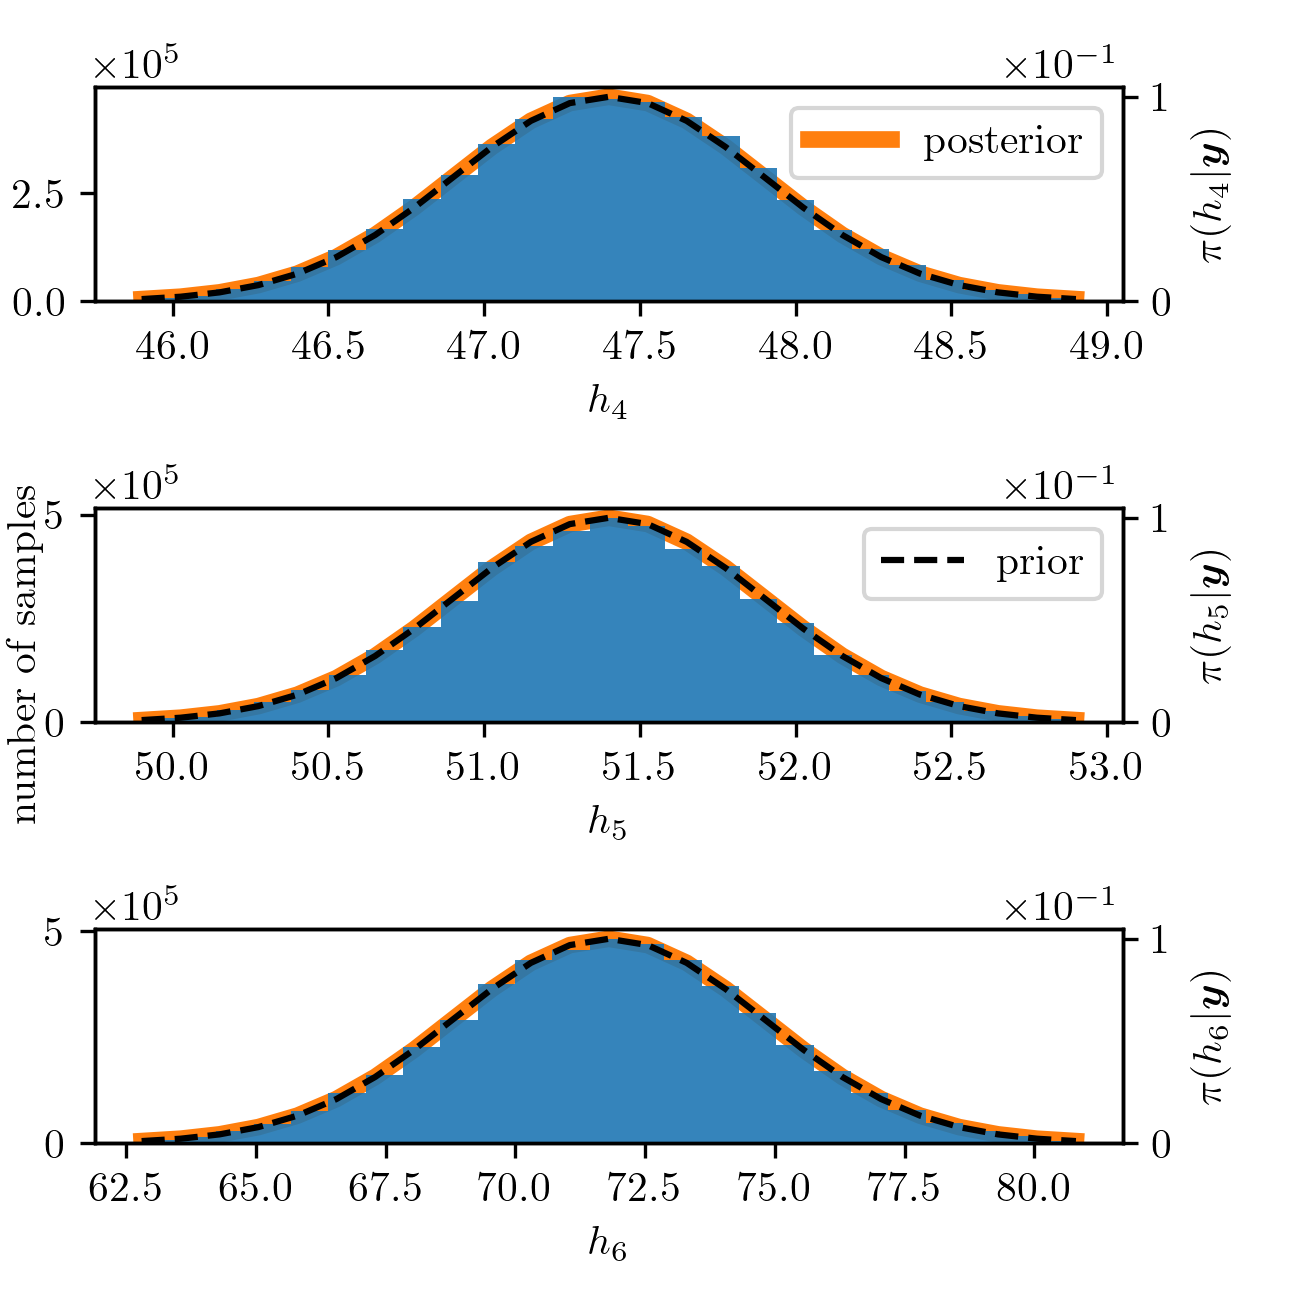
\includegraphics{PHdPTPost1.png}
	\caption[]{}
	\label{fig:PostHistTT1}
\end{figure}
\begin{figure}[ht!]
	\centering
	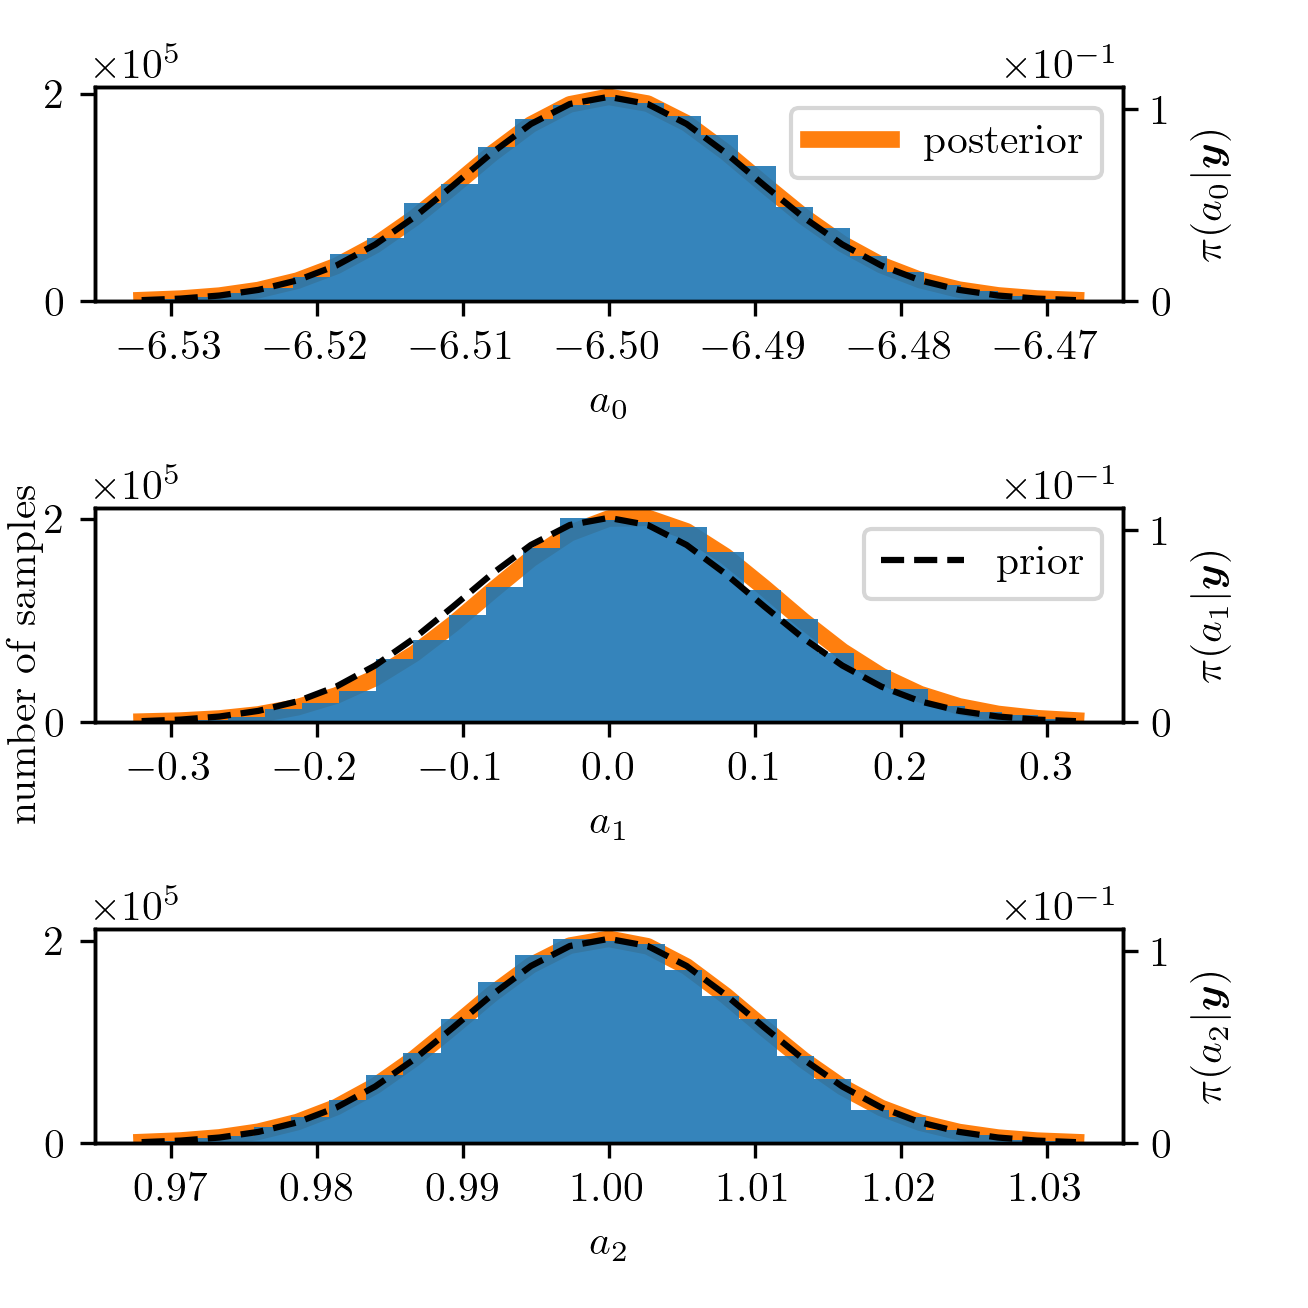
\includegraphics{PHdPTPost2.png}
	\caption[]{}
	\label{fig:PostHistTT2}
\end{figure}
\begin{figure}[ht!]
	\centering
	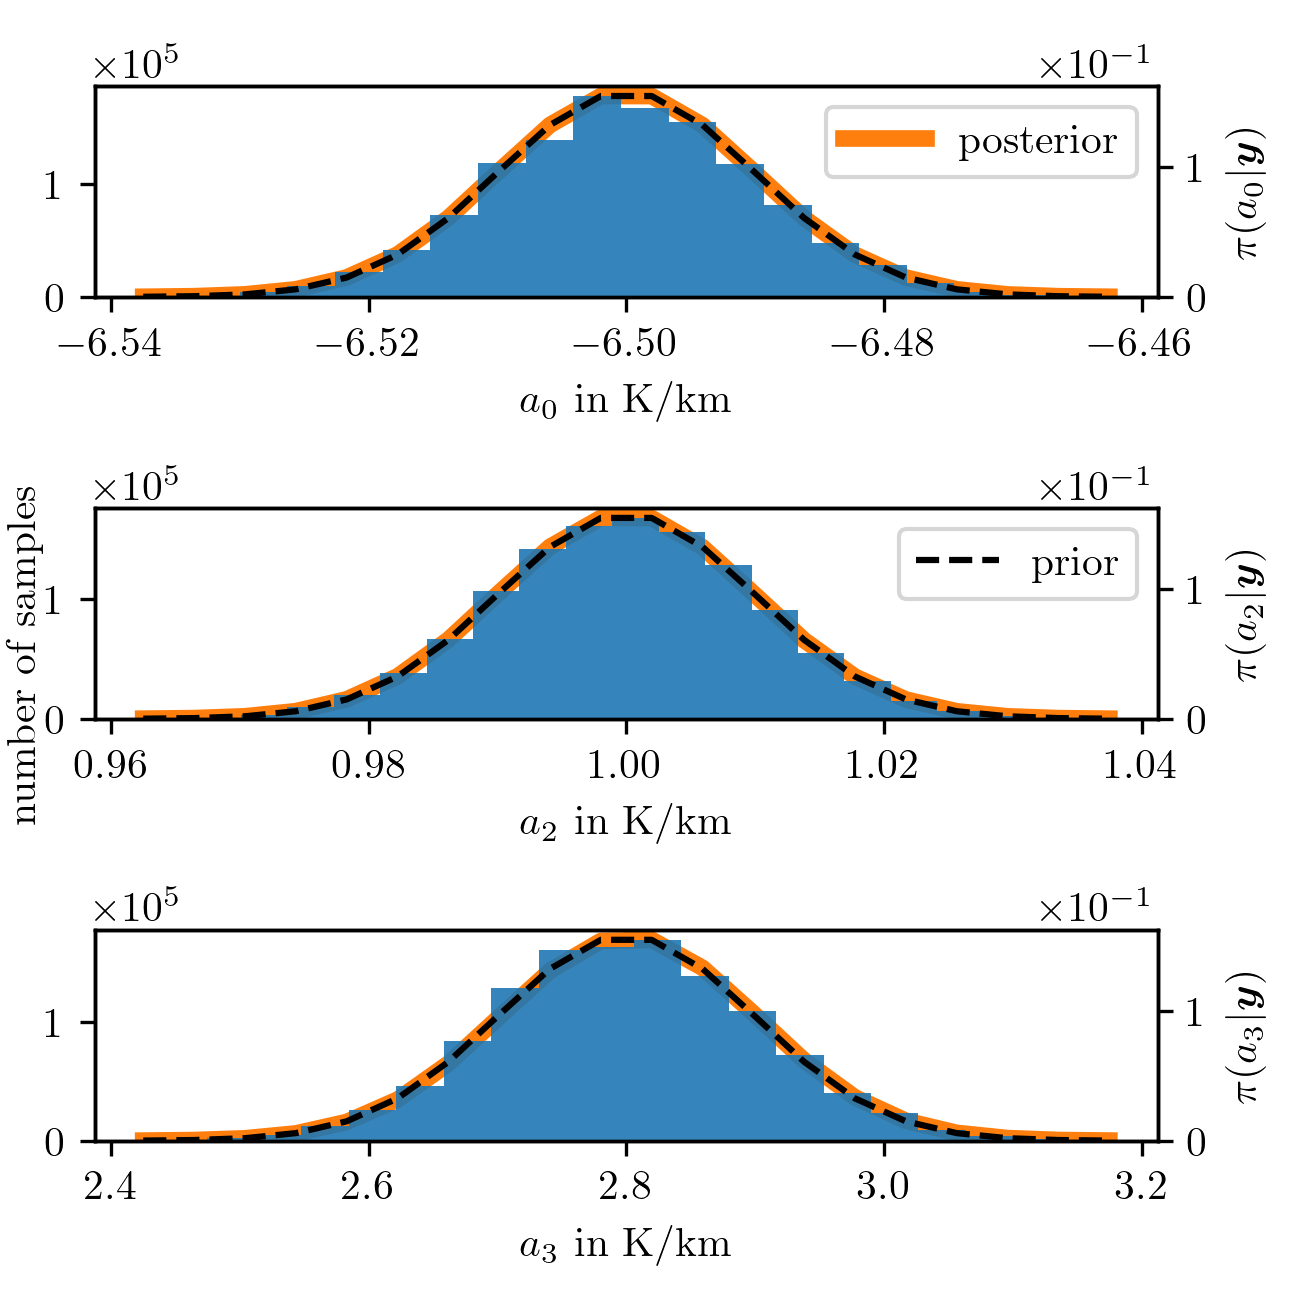
\includegraphics{PHdPTPost3.png}
	\caption[]{}
	\label{fig:PostHistTT3}
\end{figure}
\begin{figure}[ht!]
	\centering
	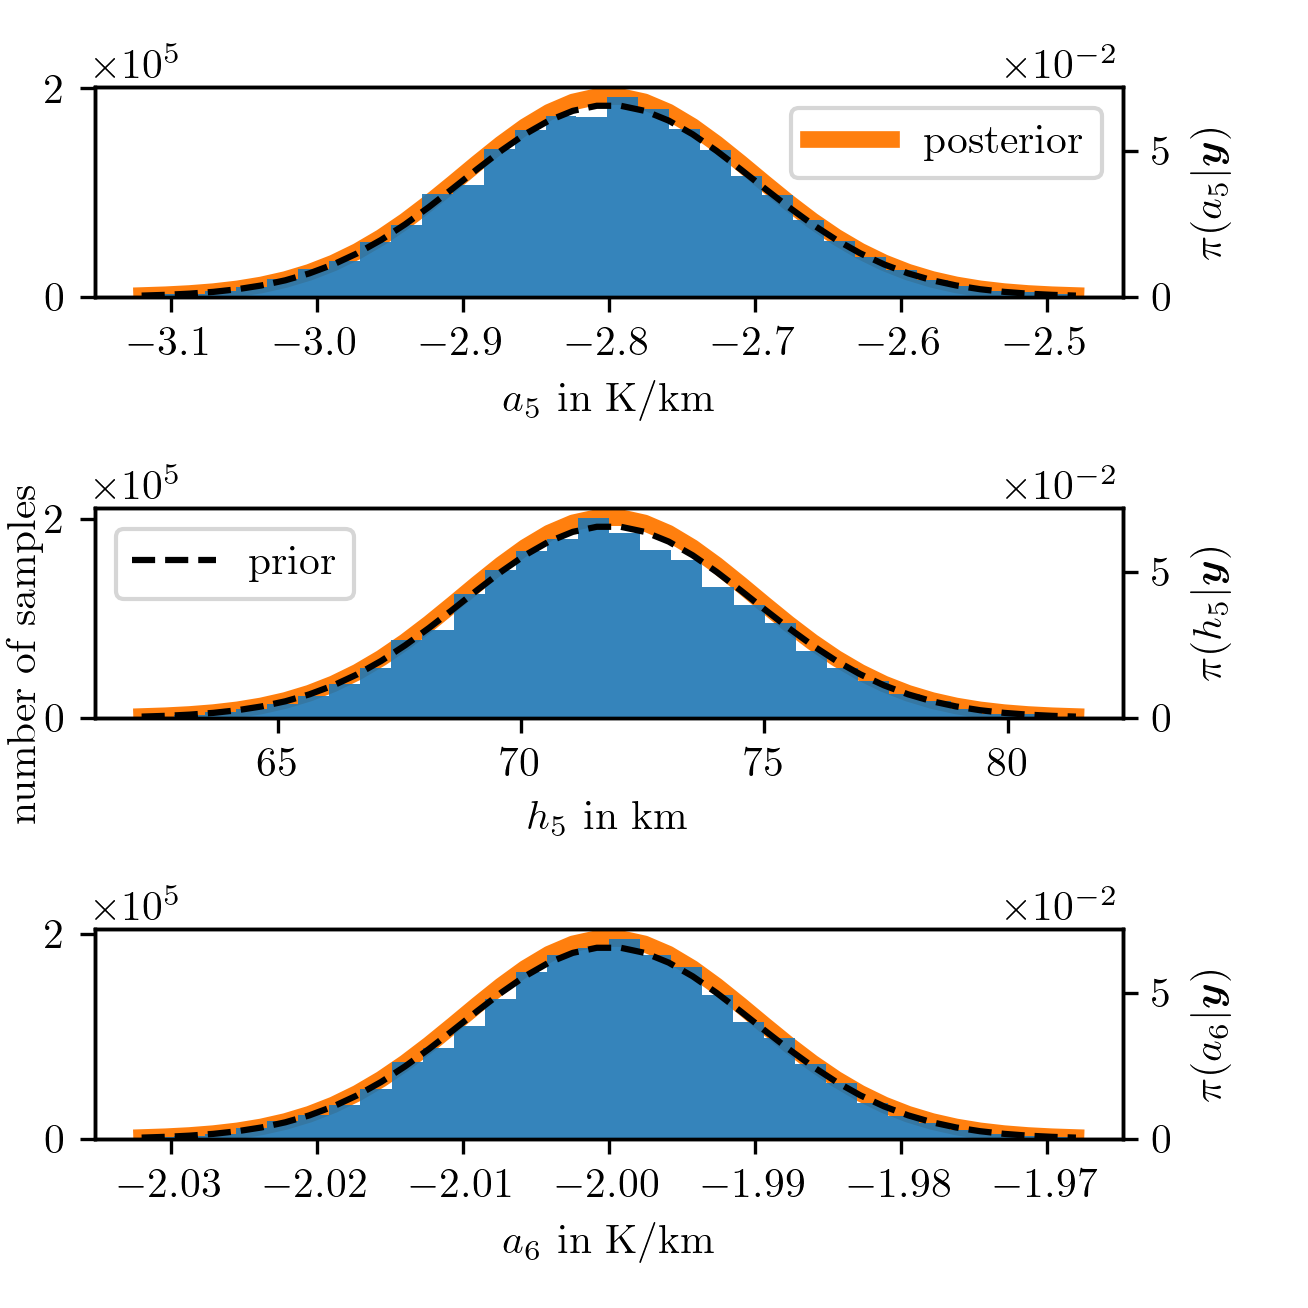
\includegraphics{PHdPTPost4.png}
	\caption[]{}
	\label{fig:PostHistTT4}
\end{figure}

\begin{figure}[ht!]
	\centering
	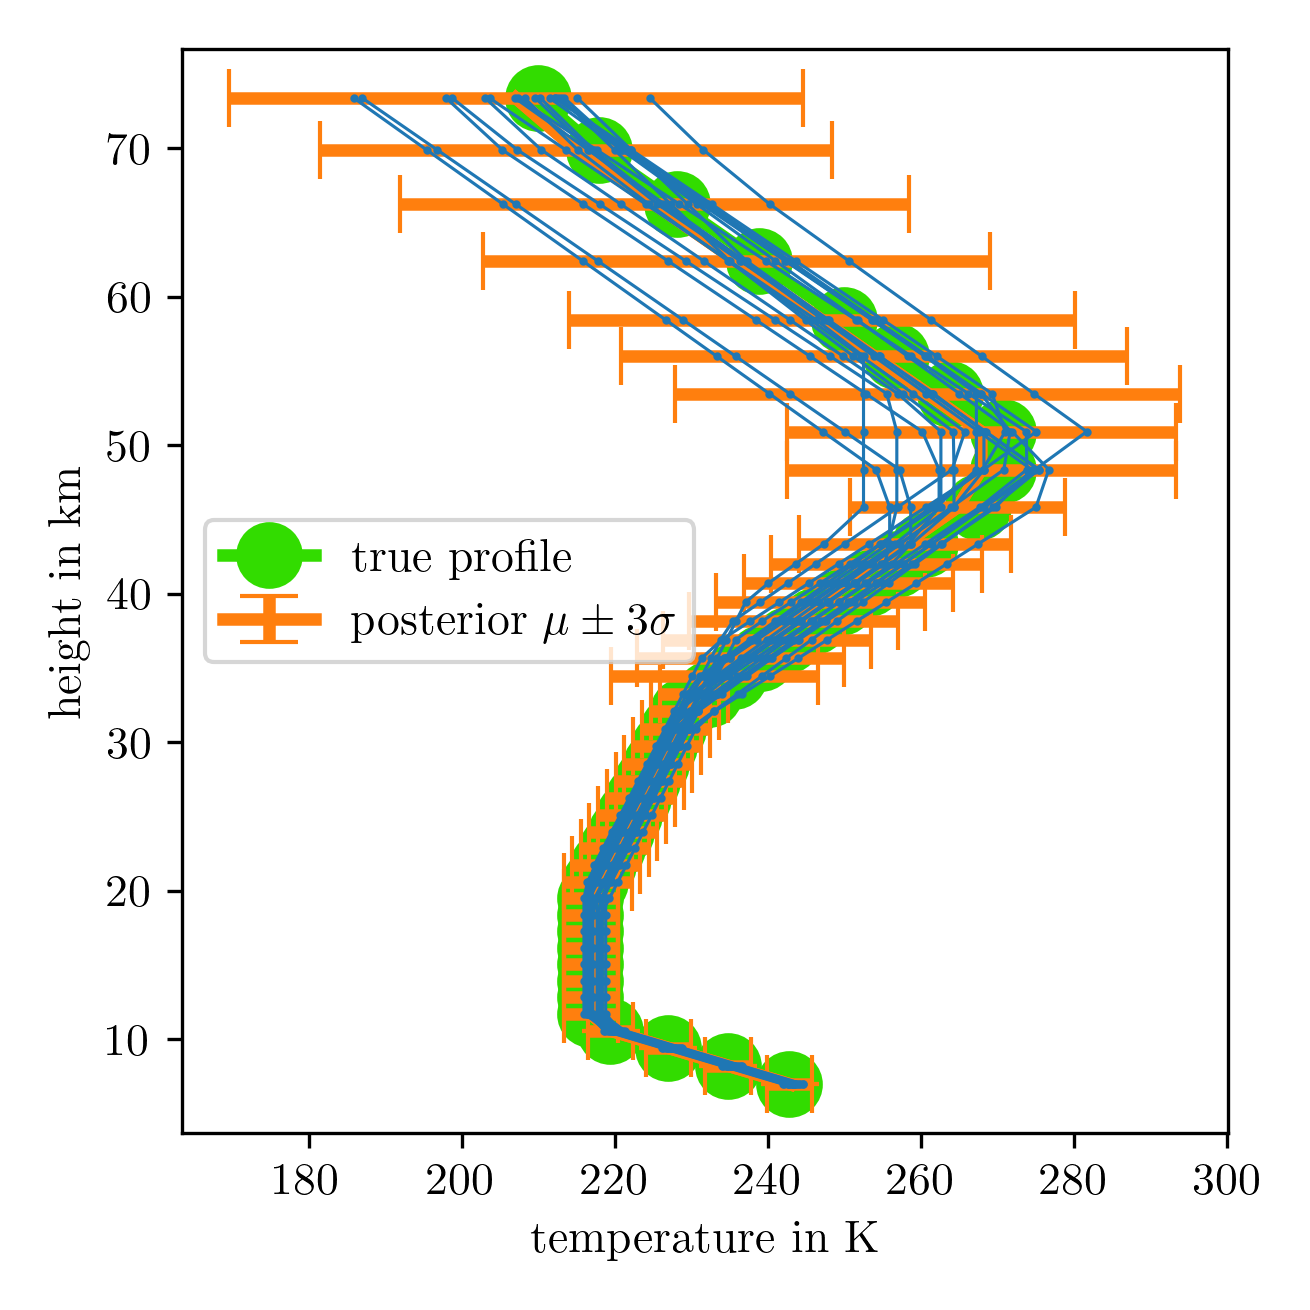
\includegraphics{TempPostMeanSigm.png}
	\caption[]{}
	\label{fig:TempPost}
\end{figure}

\begin{figure}[ht!]
	\centering
	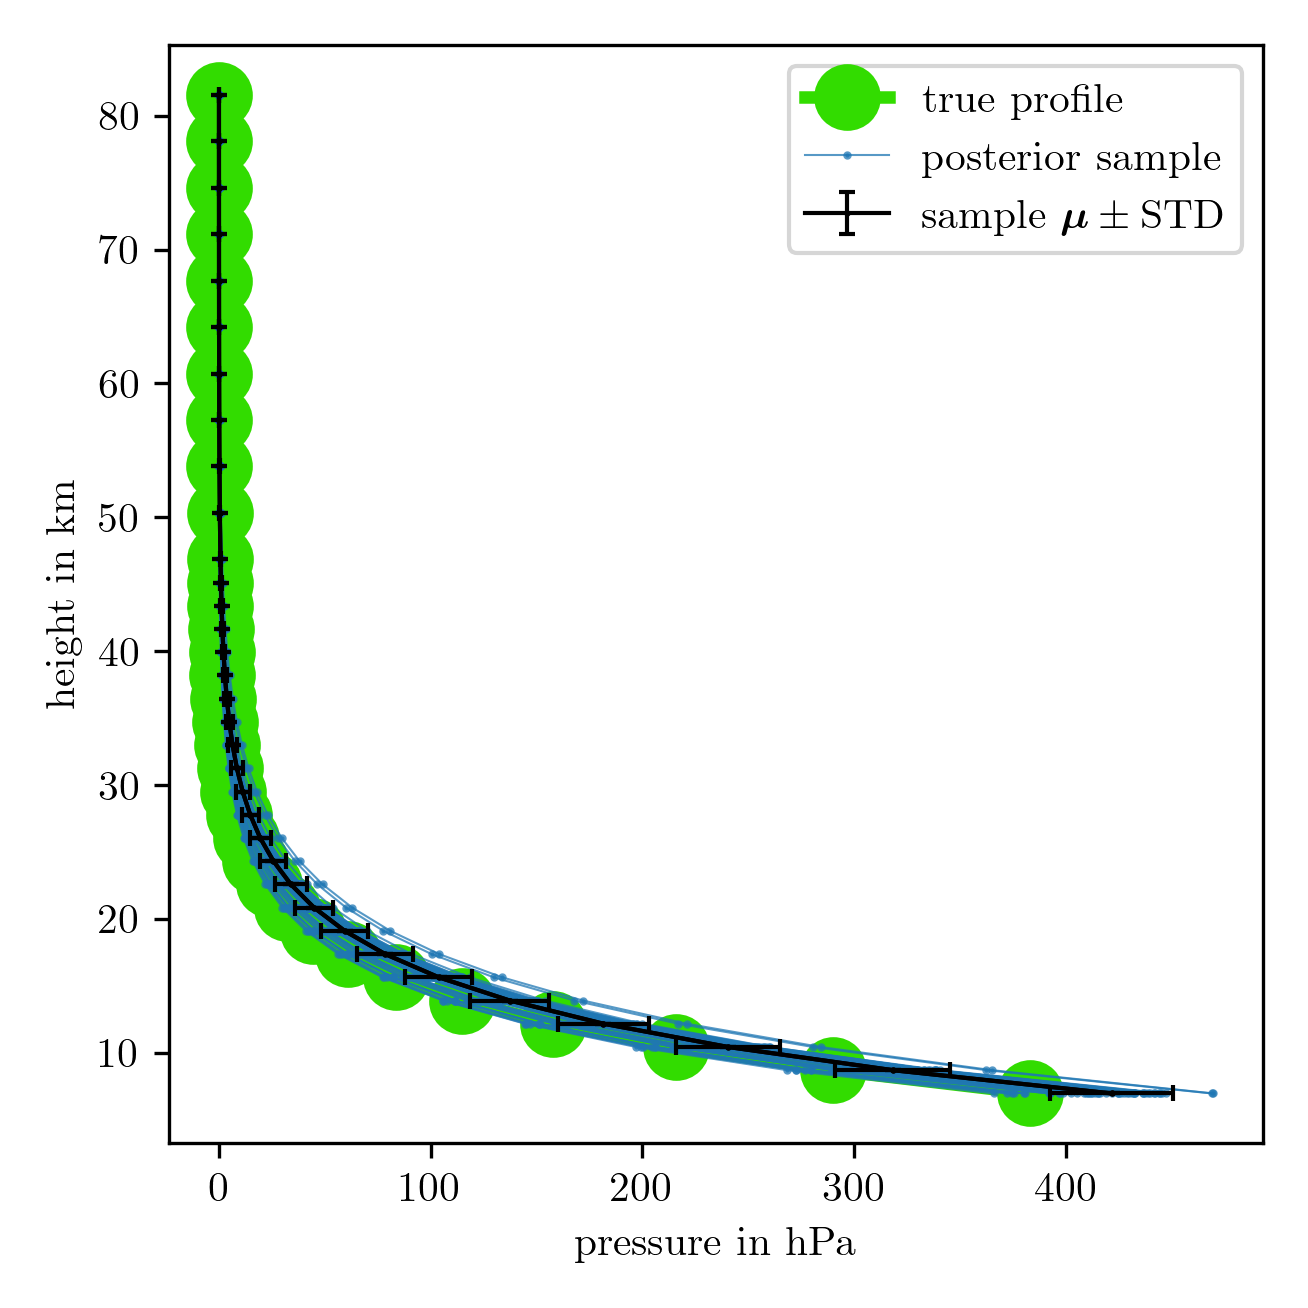
\includegraphics{PressPostMeanSigm.png}
	\caption[]{}
	\label{fig:PressPost}
\end{figure}



